\chapter{Binding energy of the $^{86}$Sr$_2$ halo molecule} \label{ch:chap5}

Weakly bound ground-state dimers are of great interest in ultracold atomic and molecular physics. 
These molecular states exhibit the strongest dependence on the long-range portion of the interaction potential between atoms.
Accurate description of the long-range part of this potential allows the scattering length, $a$, to be determined which is of the utmost importance in characterizing ultracold atomic physics.
Measurement of the binding energy precisely determines the associated $s$-wave scattering length ($a$) for free-atom collisions. 


inding energy and scattering length are inversely correlated.
Atoms with large scattering lengths will have molecular resonances nearby zero collision energy.
given by E=hma2
Plugging in the values for 86 we estimate the most weakly bound level to have a binding energy of 86 kHz.
Such extremely weakly bound molecules have special properties and are known as halo molecules.
As discussed in Chap 1, halo molecules are
Fig.\,\ref{fig:86haloWF} shows the halo state for 86

Of particular interest, the most weakly bound molecules are known as halo molecules which exhibit universality, meaning that molecular properties such as size and binding energy can be parameterized by the single quantity $a$ independent of other details of the atom-pair interaction \cite{kgj06,bha06}.



Atomic interaction potentials are difficult to understand a priori due to the complicated nature of multi-electron atoms.
Even more so in the case of two valence electron atoms such as strontium.
as we've needed to understand the potentials better, we've developed anayltic models for describing portions of the potential.
GF considered a pure van-der-waals C6 potential and found that it can be analytically solved for the binding energies.
By extending their model, they described interaction potentials that asymptote to a van-der-Waals form using an additional parameter, the van der Waals length $l_{\mathrm{vdW}}$, which defines a length scale beyond which the C6 portion of the potential dominates.
This provided a way to estimate the binding energy for weakly bound molecular states.
For system which exists near a scattering resonance, the analytic approximations of GF are expected to be quite accurate.

Efimov trimers also exist in systems near a scattering resonance, influencing dimer and atomic scattering properties and introducing additional universal phenomena \cite{bha07,nen17}.



The known scattering properties of strontium are mass scaled from 88 \hl{is this somehow not as good for 86? Also, where are the most up to date scattering lengths for Sr from?
The '10 Fourier paper} but by probing the 86 ground state potential directly we can obtain a more accurate measurement of the 86-86 scattering length.


previous chapter we explored the coupling of the intermediate state and halo state via measuring the suseceptibility as a function of the light intensity and detuning from the intermediate state.

This revealed the that it is ctrongly coupled and that our iniital experiments were in a strongly coupled regime.

In order to gain a more precise determination of the natural binding energy of the halo binding enrgy, we repeated similar expweriments as before where we varied the laser intensity at a single fixed detuning.

We also varied the trap depth to look for any differences in susceptibility between the halo state and the asymptote.


In the extreme case of a scattering resonance, the least-bound state represents an example of a quantum halo system \cite{jrf04} with spatial extent well into the classically forbidden region. 



We accurately determine the $^{86}$Sr$_2$ binding energy, considering possible collisional frequency shifts and AC Stark shifts due to trapping and excitation lasers. 
Using the universal prediction for the binding energy, including corrections derived for a van der Waals potential \cite{gfl93,gao01,gao04}, we derive a more accurate value of the $s$-wave scattering length for $^{86}$Sr atomic collisions \cite{skt10,mmp08}.

Finally, we consider the strontium interaction potential given by Tiemann.
From our measurement of the 86 binding energy we estimate the value of C6 for strontium and use a modified version of the potential to estimate imrpoved scattering lengths for all isotopes via mass scaling.



	\begin{figure} 
	\centerline{
	  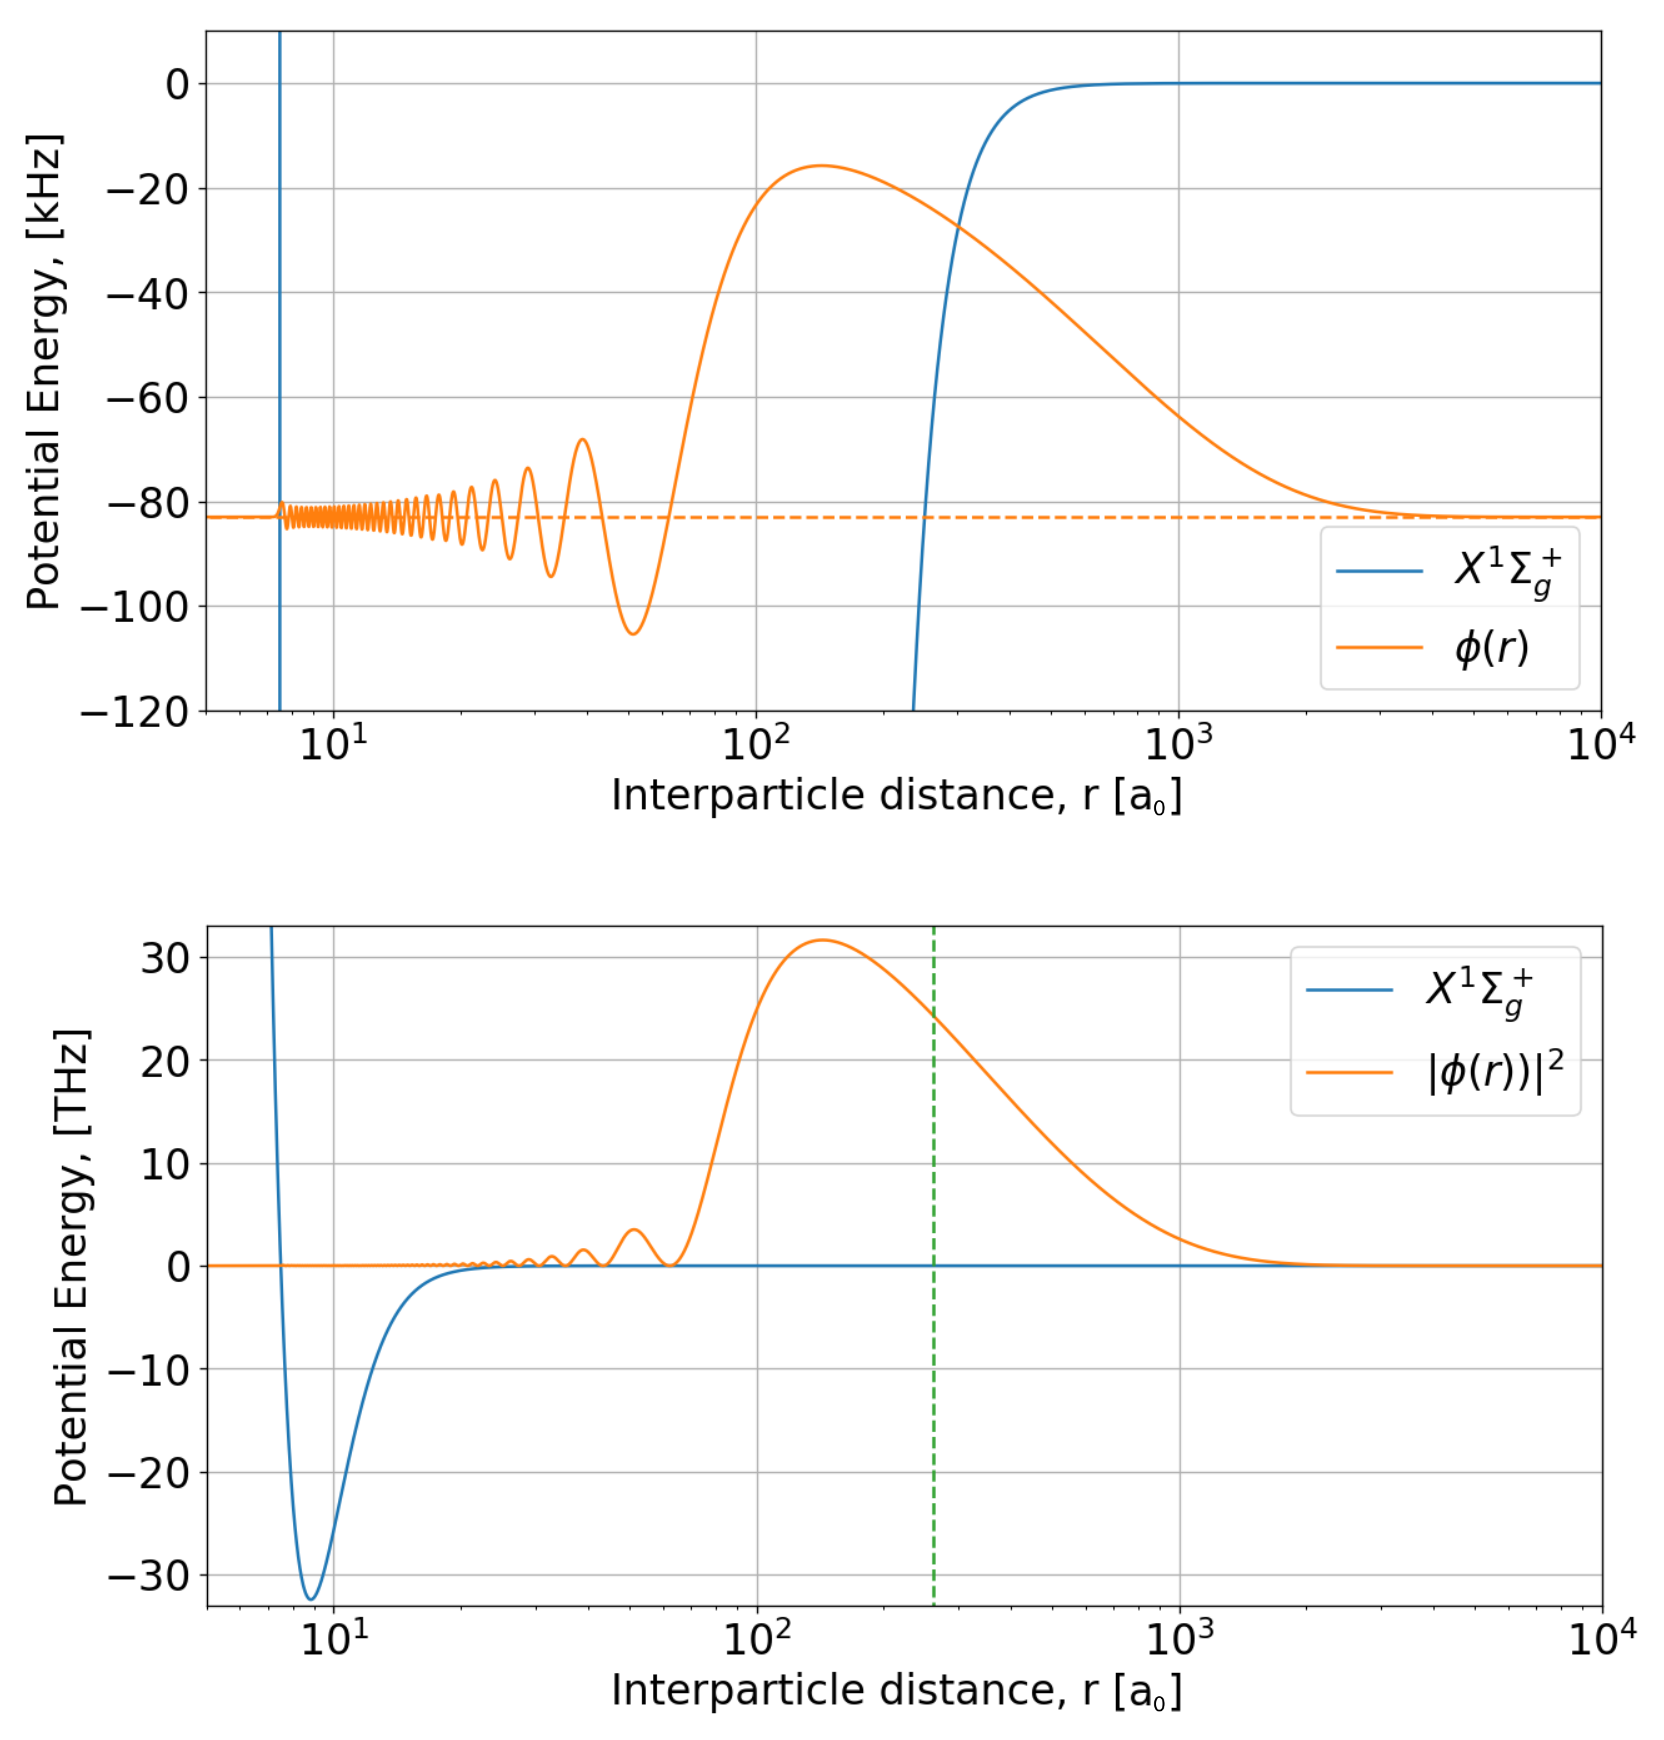
\includegraphics[width=\textwidth]{86halo.png}}
	  \caption{$^{86}Sr$ halo molecule wavefunction}{The wavefunction (top) and probability amplitude (bottom) of the halo molecule calculated using the strontium ground state potential from Tiemann \hl{ref}. Note the difference in energy scales to illustrate the weakest portion of the ground state potential. The wavefunction and probability amplitude have been scaled to be visible on each figure and are not normalized. As expected the halo molecule extends far into the classically forbidden region with the classical turning point, given by Eq.\,\hl{something}, $r_{clas} = \left( \frac{a^2 m C_6}{\hbar^2} \right)^{1/6} \approx 260\,a_0$ }
	  \label{fig:86haloWF}
	\end{figure}


	In our first experiments probing the 86 halo, prsented in the previous chapter, we probed the regime of strong coupling and observed large AC stark shifts and higher order Raman processes.
	These processes strongly perturbed the bare halo molecular state.
	Therefore, our next experiments choose to examine the weak coupling regime by applying low intensity excitations.
	This allows us to apply a simple isolated resonance model and precisely determine the effects of excitation lasers via intensity variation.
	Furthermore, we explored the 





\section{Modeling the PA spectra} \label{sec:lowE_theory}
%%%% intro
Excitation to the halo state proceeded following the same general prescription as the photoassociation experiments presented in the previous chapter.
However, the trap geometry was slightly modified to produce a larger trapping volume.
This allowed us to maintain similar overall densities compared to our previous work, while allowing variation of the trap intensity to search for a difference in the AC Stark shift at 1064\,nm between the free-atom asymptote and halo molecule state.

The single-beam optical dipole trap is generated from a 1064\,nm laser propagating perpendicular to gravity produced this high volume trap.
After forced evaporative cooling, we achiev atom temperatures between 30\,nK - 1000\,nK with typical atom numbers several hundred thousand and peak densities $\approx \peakDens{1}{12}$. 
The number of atom number and sample temperature are measured using time-of-flight absorption imaging and trap oscillation frequencies are determined by measuring dipole and breathing collective mode frequencies.



%%%% recap
As discussed in Chap 3, a description of photoassociative loss processes can be reduced to determining the inelastic loss rate coefficeint $K$.
This discussion of the rate loss constant assumed we could describe the spatial distribution of the atomic density profile analytically.
This is a valid supposition given two key assumptions, 1) the sample termperature remains constant during the PA exposure and 2) the trap is of sufficient depth that we can reasonably approximate it as a harmonic trap. \hl{cite Mi's trap paper}.
This simplifies the description of the density and velocity distributions within the trap.



result of fitting is a series of lorentzians.
energy A value causes the amplitude to grow
boltzmann factor occupation probability causes it to decrease

A discussed in the previous chapter, there are several concerns regarding the rigorous application of the Bohn and Julienne theory \cite{bju96} to these halo experiments.
The first being that it assumes an isolated intermediate state which we demonstrated breaks down as $\Delta_1$ or intensity is increased, (Fig.\hl{something}).
However, for our experiments here at fixed $\Delta_1 = +9$\,MHz and low intensities, any perturbations from additional states are expected to be neglibigle.



Need to get the full form of K from ch 4, then describe what pieces I have here. Then 


\subsection{Consideration of the trap depth} \label{sec:trunc_trap}
The trapping potential is given by $U(\mathbf{r})=mgz +h\chi_{1064,\text{g}}I_{1064}(\mathbf{r})-\tilde{U}_{\text{min}}$, where $mgz$ is the gravitational potential at height $z$, $I_{1064}(\vec{r})$ is the intensity of the trapping light, and $\chi_{1064,\text{g}}=11$\,Hz/(W/cm$^2$) \cite{YeKatori2008} is proportional to the polarizability of ground state atoms due to $1064$\,nm light.

If the single-particle kinetic-energy distribution function is a Boltzmann truncated at $U_{\text{depth}}-U(\mathbf{r})$, then the collision-energy distribution follows a Boltzmann distribution at low energies $[\epsilon\ll U_{\text{depth}}-U(\mathbf{r})]$ and falls off more quickly at larger energies, reaching zero at $2[U_{\text{depth}}-U(\mathbf{r})]$.





Three effects to discuss, the non analytic density distribution, the truncation of the energy, and the non-ergodicity.
Density distribution because we need to know the spatial weighting at each position in space.
Truncation of energy because the position in space leads to a spatially dependent maximum kinetic energy.
The non-ergodicity because it means we don't actually know what the maximum kinetic energy should be.

%%%% Density distribution
This provides an analytically simply relationship between the spatial coordinates and the atoms potential energy due to the trapping potential.
Such a description is typically valid when the ratio of the trap depth to the sample temperature is $>4$, as shown in appendix.
We define this ratio to be $\eta = U_{\text{depth}}/k_B T$.

Second, we consider the spatial density profile of the atomic sample and consider the number of atoms available in each region of the cloud.


%%%% Energy truncation
In a typical high-eta trap, a Boltzmann profile is sufficient to describe the velocity distribution of the atoms and when we consider the distribution of relative energies that is important for PAS expeirments, we recover a simple bolztmann weighting for the distribution of energy probabilities. 
This is shown in \hl{sopme app}.

Then we have to figure out the distribution of collision energies.
Following the example in \hl{ref}, chapter 3 considers two additional albeit related effects.

First, we consider the truncation of the collision energy interval.
For traps of finite depth, we expect each atom to have kinetic energy up to $U_{\text{depth}}/k_B T$.
We define this ratio as the trap-$\eta = U_{\text{depth}}/k_B T$.
Therefore, the maximum collision energy is $2\eta$ between two particles each with kinetic energy $\eta$.

shift of the ground state energy by the trapping potential for each shell of density.


%%%% Non-erogdicity
decide to fit both 1ud and 2ud as limiting cases because we aren't sure which energies contribute to the atomic loss





$\tilde{U}_{\text{min}}$ is subtracted to set the potential at the trap minimum to zero. The spatial integral is restricted to regions around the trapping local minimum with $U(\mathbf{r})$ less than the trap depth \cite{ycm11}.

Downhill regions on the other side of the saddle point defining the trap depth are excluded. The laser intensity profile is measured independently, and the potential is found to be consistent with measured trap oscillation frequencies.

The partition function is $Q_{T}=\left({2\pi k_{B}T \mu \over h^2}\right) ^{3/2}$ for reduced mass $\mu=m/2$ and sample temperature $T$, for atoms of mass $m$.

Equation (\ref{equationKeffective}) provides the correct thermal average when the collision-energy distribution does not need to be truncated $(\epsilon_{\text{max}}\rightarrow \infty)$.

For our data, however, the ratio of sample temperature to trap depth is $k_BT/U_{\text{depth}}\approx 3$ for samples with temperature above $100$\,nK and drops to unity for 30\,nK samples, so truncation effects are important.

We find that this treatment predicts a narrower distribution on the red side of the spectral line than we observe in our data, suggesting the presence of atoms in non-ergodic orbits with energies above the saddle point of the trap.

This is not surprising given the large collisional loss rate associated with near-resonant scattering in this isotope.




Analysis of the trapping conditions following acquisition of the PAS data revealed that this second assumption was not maintained during these low-intensity experiments.
Lacking an analyitic expression for the density distribution, a description of the bulk properties is possible by discretizing the trap and considering it's local properties.
Fig.\,\ref{fig:haloTrapModel} shows the potential energy surface for a characteristic trap used in this experiment.
Recalling that the trap depth is defined between the trap minimum and the lowest saddle point, we see that this point is along a non-trivial trajectory.
Thus atoms at high kinetic energies may remain trapped in the region and the timescale to reach equilibrium is long.
	\begin{figure} 
	\centerline{
	  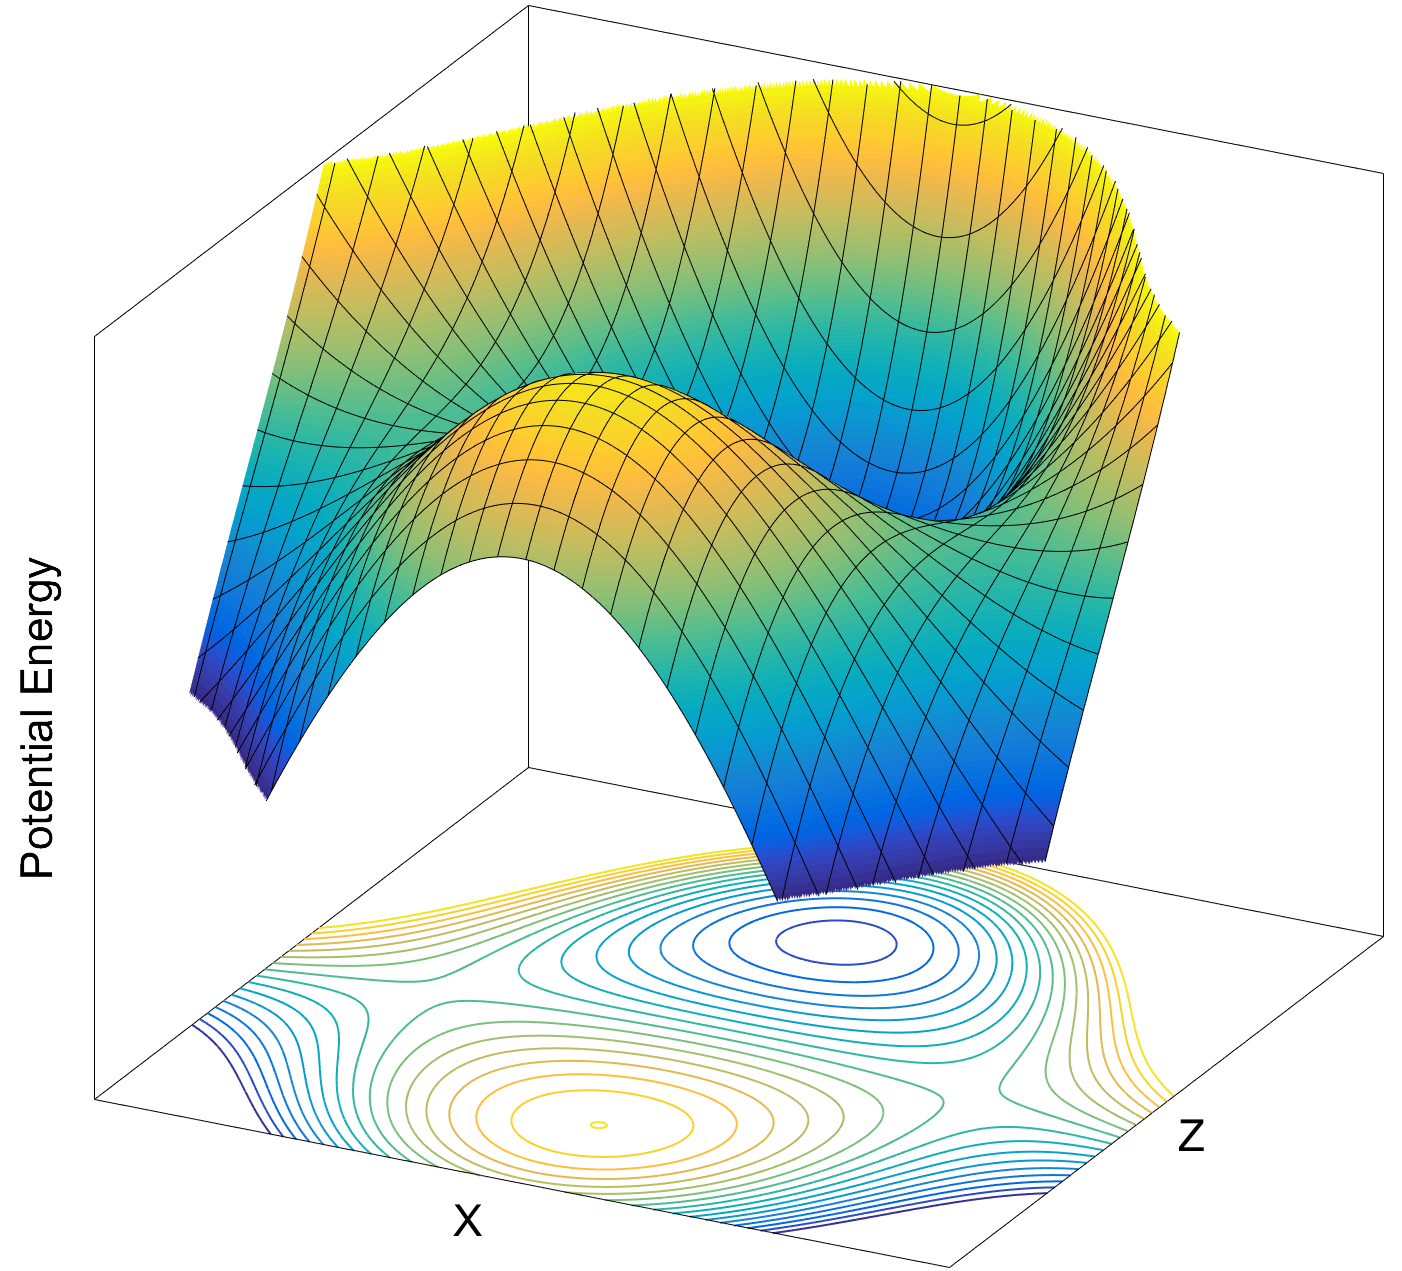
\includegraphics[width=\textwidth]{haloTrapV2.png}}
	  \caption{Surface plot of the trapping volume in single beam trap}{The spatial dependence along the XZ plane with Y=0 of the ground state potential energy during the halo molecule excitation. Note, this coordinate system assumes the laser wavevector is propagating along +X and gravity is aligned along -Z. We can clearly see the trap depth is defined along a trajectory where a particle is simultaneously moving away from the beam waist and down under the influence of gravity.}
	  \label{fig:haloTrapModel}
	\end{figure}
Due to this ambiguity

In addition to the modified spatial distribution, we must also consider the effect of the trap depth on the energy profile of the trapped gas.

This is troublesome as it means we must numerically consider the density distribution over space when solvinf for the rate loss constant K. 

However, the case of a low-eta trap we must define a local cutoff energy at each point in space within the trap as atoms that have an energy higher than the local eta value are assumed to be lost from the trap.



Derivation of this truncated relative energy probabillity distribution is given in \hl{some app} and results in a stronger weighting of the coldest atoms near the bottom of the trap.
	\begin{figure} 
	\centerline{
	  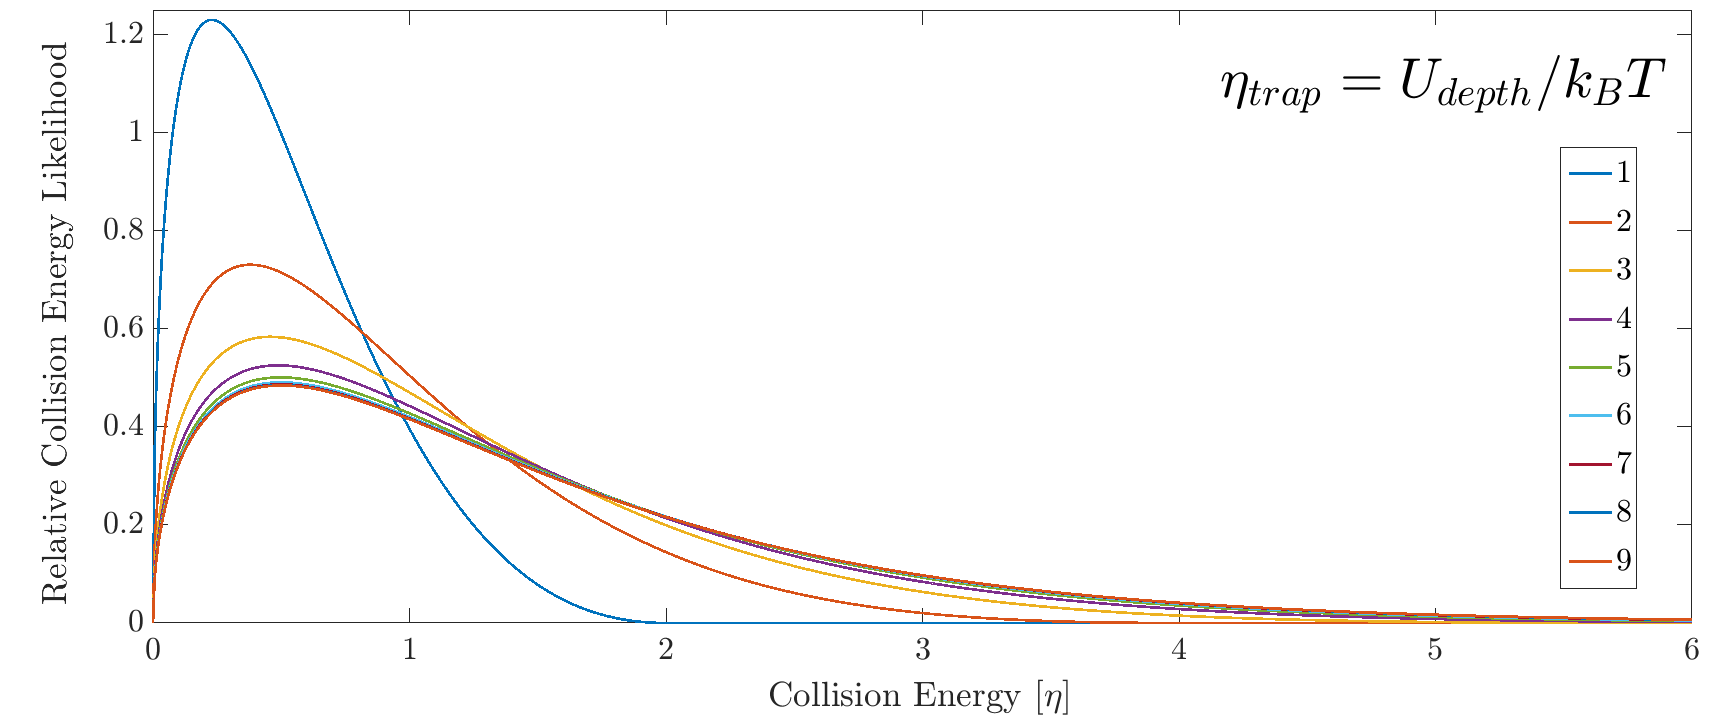
\includegraphics[width=\textwidth]{1DrelativeCollProbvsCollEn.png}}
	  \caption{Relative collision energy distributions for various trap depths}{The effects of energy truncation on the likelihood of collisions at different various trap depths where the total collision probability for each curve is normalized to unity. Energy is specified in units of $\eta = U_d/k_B T$. Each trap has a maximum collision energy of $2\eta_{trap}$ between two particles each with maximum kinetic energy $\eta$.}
	  \label{fig:relativeCollProb}
	\end{figure}
For deep traps, the effects of the energy truncation due to the finite trap depth become negligible and the relative collision energy likelihood approaches a Maxwell-Boltzmann.
Details of this limiting behavior are given in App.\,\ref{app:mom}.


\subsection{Fitting the thermally averaged spectra} \label{sec:lowIntSpectra}



Fortunately, the molecular binding energy is strongly determined by the sharp edge of the spectrum on the blue side of the line, which is relatively insensitive to the description of the red tail.

Our data is fit well with a truncated Boltzmann distribution of collision energies [Eq.~(\ref{equationKeffective})].

To estimate the systematic uncertainty introduced by this treatment, we perform fits with $\epsilon_{\text{max}}$ equal to $2[U_{\text{depth}}-U(\mathbf{r})]$ and $U_{\text{depth}}-U(\mathbf{r})$ and take the mean of the two results as the best value for the binding energy and half the difference as a systematic uncertainty $\sigma_{\epsilon_{\text{max}}}\approx 100$\,Hz.

This procedure does not correctly represent the overall normalization of $\langle K \rangle$, but we are not concerned with overall signal amplitude in this study.

Atom temperatures vary by no more than 20\% during the interaction time, so assuming a constant sample temperature is reasonable.




In Ch. \hl{somewhere} we discussed the usual situation for observing loss due to photoassocition. 
This experiment was similar to the 88 autler townes experiment. 

	\begin{figure} 
	\centerline{
	  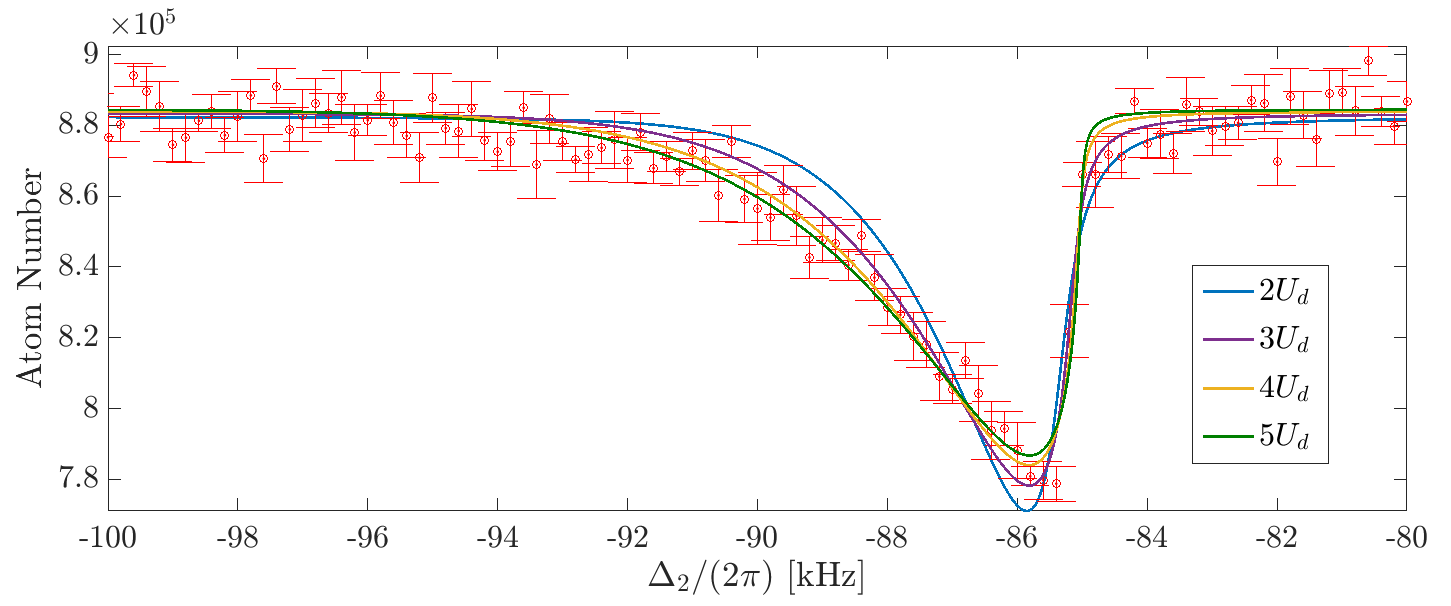
\includegraphics[width=\textwidth]{truncated_fixU_compare.png}}
	  \caption{Comparison of lineshape fits at various $\epsilon_{\text{max}}$}{Using a constant trap geometry (eg. Fig.\,\hl{trapFig}) with a trap depth $U_d$, the spectra is fit with varying maximum collision energy, $\epsilon_{\text{max}}$. The solid lines give the maximum single particle kinetic energy such that the collision energy is twice  Temperature of this sample is 100\,nK}
	  \label{fig:truncatedSpectraFit}
	\end{figure}
Two notable features, 1) the linewidth on the right side starts broad and becomes more narrow as the maximum collision energy is increased.
Conversely, the 

these are fits so when the model is not appropriate the algorithm will broaden out the line and shift the binding energy to try and describe the data.
For max coll of 2, we see a broad linewidth was 

The tail is given by atoms near the center of the trap. These are high enegy atoms which are only possible 

this data did not show an increase in tmperature and the timescales used are apprpriate for a frozen gass approximation.
The hotest atoms must be near the center of the trap since this is the only region deep enough to keep them trapped.
Converely, cold atoms appear nea the edges of the trap for the same reason.
Thus we can see that for a max collision energy of 2U, the linewidth biases towards large values and the binding energy shifts. This si suggestive that the model is incomplete at his energy and we are missing contrributions from hotter atoms.
As we increase the maximum collision energy, the linewidth decreases and begins to better describe the observed data. At the same time, we begin accurately accounting for the thermal portion of the spectrum.
Since it is not clear which description is most acurate for our scenario, we choos eto fit the data at the limits of 2U and 4U as shown in Fig. something.







Bohn and Julienne \cite{bju96} provide an expression for $\vert S(\epsilon,\omega_1,\omega_2,...)\vert^2$ for a collision on the open channel of two ground state atoms (g) with total energy $\epsilon$ leading to loss-producing decay from the excited state $b_1$ with rate $\gamma_1$ (Fig.\ \ref{PASDiagram}),
\begin{eqnarray}
  \vert S\vert^2 =   \hspace{2.5in}&&\\
  {(\Delta_2+\epsilon/\hbar)^2{\gamma}_1{\gamma}_s \over
  	\left[(\Delta_1+\epsilon/\hbar)(\Delta_2+\epsilon/\hbar)-\frac{\Omega_{12}^{2}}{4}\right]^2+\left[ \frac{\gamma_1+\gamma_s}{2}\right]^2(\Delta_2+		 	\epsilon/\hbar)^2}. &&\nonumber
\end{eqnarray}


For simplicity, we have omitted the light shift of $b_1$ due to coupling to the scattering continuum \cite{bju99}.

This approach was found to be sufficient for describing two-photon spectroscopy to a more deeply bound molecular level in $^{88}$Sr \cite{mmp08}.

Equation (\ref{equationSprob}) neglects all light shifts due to the trapping laser. Light shifts due to the photoassociation lasers coupling to states outside our model (Fig.\ \ref{PASDiagram}) are also neglected.

The thermal energy is much greater than the zero-point energy for trap motion, $T\gg h\nu_{\text{trap}}/k_B$, so confinement effects are negligible \cite{zbl06}.

${\gamma}_{1}=2\gamma_{\text{atomic}}$, where $\gamma_{\text{atomic}}=4.7\times 10^4$\,s$^{-1}$ is the decay rate of the atomic $^3P_1$ level.

${\gamma}_{s}(\epsilon)$ is the stimulated width of $b_1$ due to coupling to the initial scattering state by laser 1, which for low energy can be expressed as \cite{ctj06,bmc14,Pachomow2017a}
\begin{equation}\label{equationstimulatedwidth}
	{\gamma}_{s}(\epsilon)=2k l_{\text{opt}} \gamma_1,
\end{equation}

where the optical length ($l_{\text{opt}}\propto I_1$) is related to the overlap between the initial colliding state and $b_1$, and $k=(2\mu \epsilon)^{1/2}/\hbar$.

We take the intermediate state $b_1$ as the $\nu=-2$ state, for which $l_{\text{opt}}/I=(1.5\pm0.3)\times 10^4\,a_0\mathrm{/(W/cm^2)}$ \cite{bmc14}, where $a_0=5.29\times 10^{-11}$\,m is the Bohr radius.

For the experiments reported here, we maintain significant intermediate-state detuning, $\Delta_1$, for which $|\Delta_1|\gg |\Omega_{2,12}|$.

Thus we are in a Raman configuration, and not in the Autler-Townes regime \cite{mmp08}.

In the Raman regime, Eq.\ \ref{equationSprob} shows a maximum near two-photon resonance at $\Delta_2+\epsilon/\hbar =\Omega_{2,12}^2/4\Delta_1$.

Following a treatment discussed recently for a similar experiment in calcium \cite{Pachomow2017a}, if the detuning is restricted to near two-photon resonance then $\vert S\vert^2$ can be approximated as a Lorentzian
\begin{eqnarray}
 \vert S\vert^2 \approx {A(\epsilon) \over
 \left(\Delta_2+\epsilon/\hbar-\frac{\Omega_{12}^{2}}{4(\Delta_1+\epsilon/\hbar)}\right)^2+\left[ {\Gamma_L(\epsilon)}/{2}\right]^2},
\end{eqnarray}
where 
%$A$ and $\Gamma_L$ are defined in Eqs.\ (\ref{ApproxLorentzianQuantitiesMain}) and (\ref{ApproxLorentzianQuantities-2Main}).
\begin{eqnarray}\label{ApproxLorentzianQuantitiesMain}
  A(\epsilon)&=& \frac{\Omega_{2,12}^{4}\gamma_1 \gamma_s(\epsilon)}{16(\Delta_1+\epsilon/\hbar)^4} \\
  \label{ApproxLorentzianQuantities-2Main}
  \Gamma_L(\epsilon)&=& \frac{\Omega_{2,12}^{2}[\gamma_1 +\gamma_s(\epsilon)]}{4(\Delta_1+\epsilon/\hbar)^2}.
\end{eqnarray}

In the absence of a more complete theory treating these effects, we analyze loss spectra using the effective expression given by Eq.\ (\ref{equationApproxLorentzian}), where the observed molecular binding energy ($E'_{b2}$) includes any perturbations due to AC Stark or collisional shifts.
\vbox{
\begin{eqnarray}\label{equationApproxLorentzian}
  \vert S\vert^2 = \frac{\Gamma_L(\epsilon)+\gamma_{\text{eff}}}{\Gamma_L(\epsilon)}\hspace{1.5in} \nonumber \\
  \times \frac{\eta  A(\epsilon)} {\left(\omega_1-\omega_2+\epsilon/\hbar-E'_{b2}/\hbar\right)^2+\left[
  	\frac{\Gamma_L(\epsilon)+\gamma_{\text{eff}}}{2}\right]^2},
\end{eqnarray}}







Parameters have been added in Eq.\ (\ref{equationApproxLorentzian}) to account for deviations of the signal strength ($\eta$) and width ($\gamma_{\text{eff}}$) from the predictions of \cite{bju96}.

If deviations from Eq.\ (\ref{equationSprobLorentzian}) are small, we expect $\eta\sim1$, $\gamma_{\text{eff}}\sim 0$, and $E'_{b2}\sim E_{b2}+{\Omega_{2,12}^{2}}/{4(\Delta_1+\epsilon/\hbar)}$.

Light shifts (AC Stark shifts) due to the trapping lasers and collisions with ground-state atoms (density $n$) should contribute to shifts of molecular resonance.

Similar effects were taken into account in a recent, high-precision study of weakly bound molecular states of ultracold ytterbium atoms \cite{bbc17}.

In addition, we expect that both 689-nm excitation lasers will shift the line, not just $I_2\propto \Omega_{2,12}^{2}$. We model the relationship between the measured resonance positions and the unperturbed binding energy $E_{b2}$ as
\begin{equation}\label{Eq:GlobalFit}
	E'_{b2}=E_{b2}+h\chi_{689}I_{689}+h\chi_{1064}I_{1064}(\mathbf{r})+h\chi_{n}n(\mathbf{r}).
\end{equation}


	\begin{figure} 
	\centerline{
	  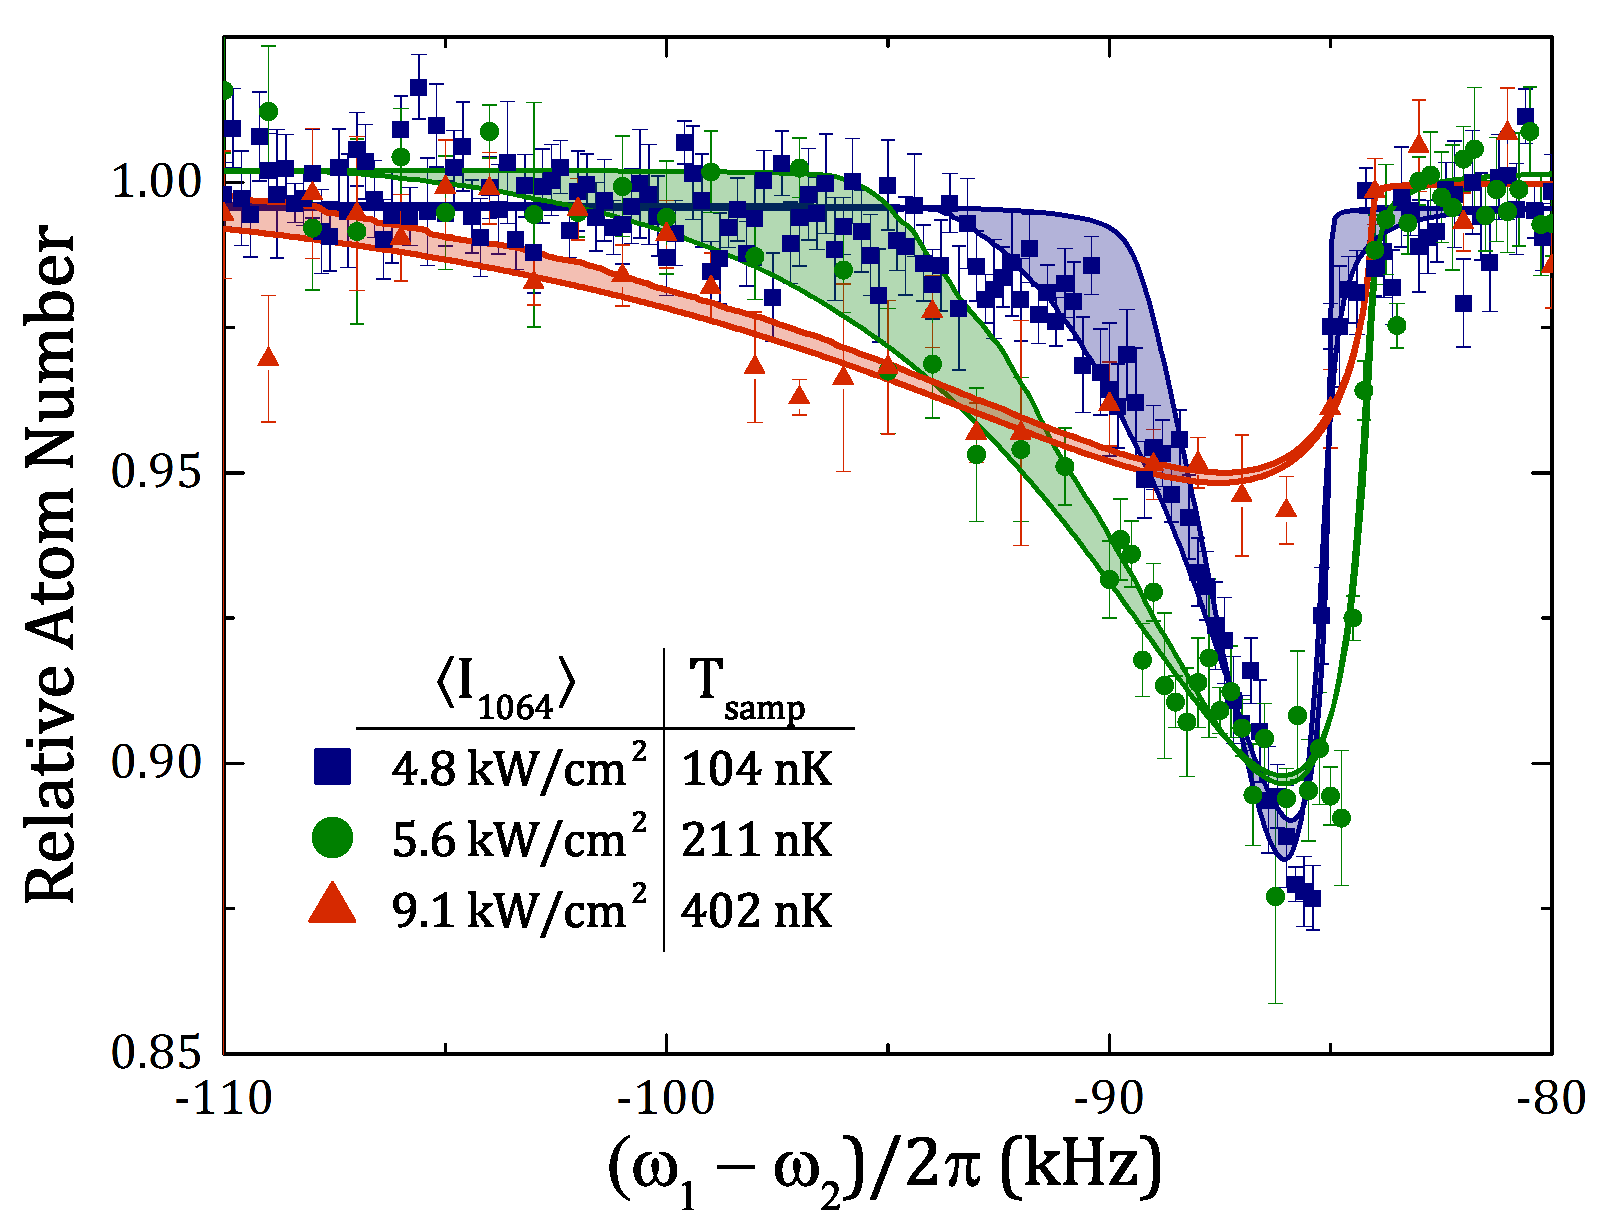
\includegraphics[width=\textwidth]{spectra_vary_1064.pdf}}
	  \caption{Variation of 1064 nm trap depth}{Atom-loss spectra as a function of two-photon difference frequency $(\omega_1-\omega_2)/2\pi$ for intermediate detuning
	$\Delta_1/2\pi=-9$\,MHz . Sample temperature and average trapping laser intensity are indicated in the legend. The single-beam excitation laser intensity is $I=25$\,mW/cm$^{2}$ for the 104\,nK spectrum and $I=48$\,mW/cm$^{2}$ for the 211\,nK and 402\,nK spectra. Fits are described in the text, with the two boundaries of each band given by the fits with collision-energy truncation
	$\epsilon_{\text{max}}$ equal to $2[U_{\text{depth}}-U(\mathbf{r})]$ and $U_{\text{depth}}-U(\mathbf{r})$.}
	
	\label{Fig:Spectraminus9MHzVaryTrapCold}
	\end{figure}












\section{Determination of energy shifts}
\label{sec:lowE_Eb2}

%% paper
%The excitation intensity is $I=0.10$\,mW/cm$^{-2}$ and the intermediate detuning is
%$\Delta_1=-9$\,MHz.
%The peak intensity for the optical dipole trap at the end of the evaporationis indicated in the figure, along with the
%peak initial sample density at the beginning of laser excitation.

Figure \ref{Fig:Spectraminus9MHzVaryTrapCold} shows a series of spectra for different final trap depths and sample temperatures.

The characteristic asymmetric lineshape for excitation of a thermal sample is evident, with width decreasing as sample temperature decreases.

The molecular binding energy is close to the sharp edge on the blue side of each spectrum.

We fit atom-loss spectra with Eq.\ (\ref{number}) for the evolution of atom number with time, using the phenomenological expression Eq.\ (\ref{equationApproxLorentzian}) for the scattering probability and Eq.\ (\ref{equationKeffective}) for the average of the collision event rate constant over the trap volume and collision energy.

The sample temperature, perturbed resonance frequency $E'_{b2}$, $\eta$, and $\gamma_{\text{eff}}$ are taken as fit parameters. 

In the final analysis, temperatures are set to values determined from time-of-flight imaging of the atoms, but when they are allowed to vary, the fit values differ by no more than 10\%.

Approximately 10 spectra are recorded for each set of experimental parameters, and the spread of resulting fit values are used to determine best values and uncertainties.


The susceptibilities, in Hz per unit intensity or density, will be determined from experimental data or theoretical considerations.

The variation with position of the trapping laser intensity ($I_{1064}$) and the density give rise to the spatial dependence of $|S|^2$ and the need for a spatial average in Eq.\ (\ref{equationKeffective}).

We take $I_{689}$ as twice the single-beam intensity $I_{689}=2I$. The 689-nm excitation beam is large enough compared to the atom sample to neglect spatial variation.

The functional form for the AC Stark shift due to the excitation lasers is discussed in Sec.\ \ref{sectionACStark}.


\subsection{AC Stark shift due to excitation lasers}

	\begin{figure} 
	\centerline{
	  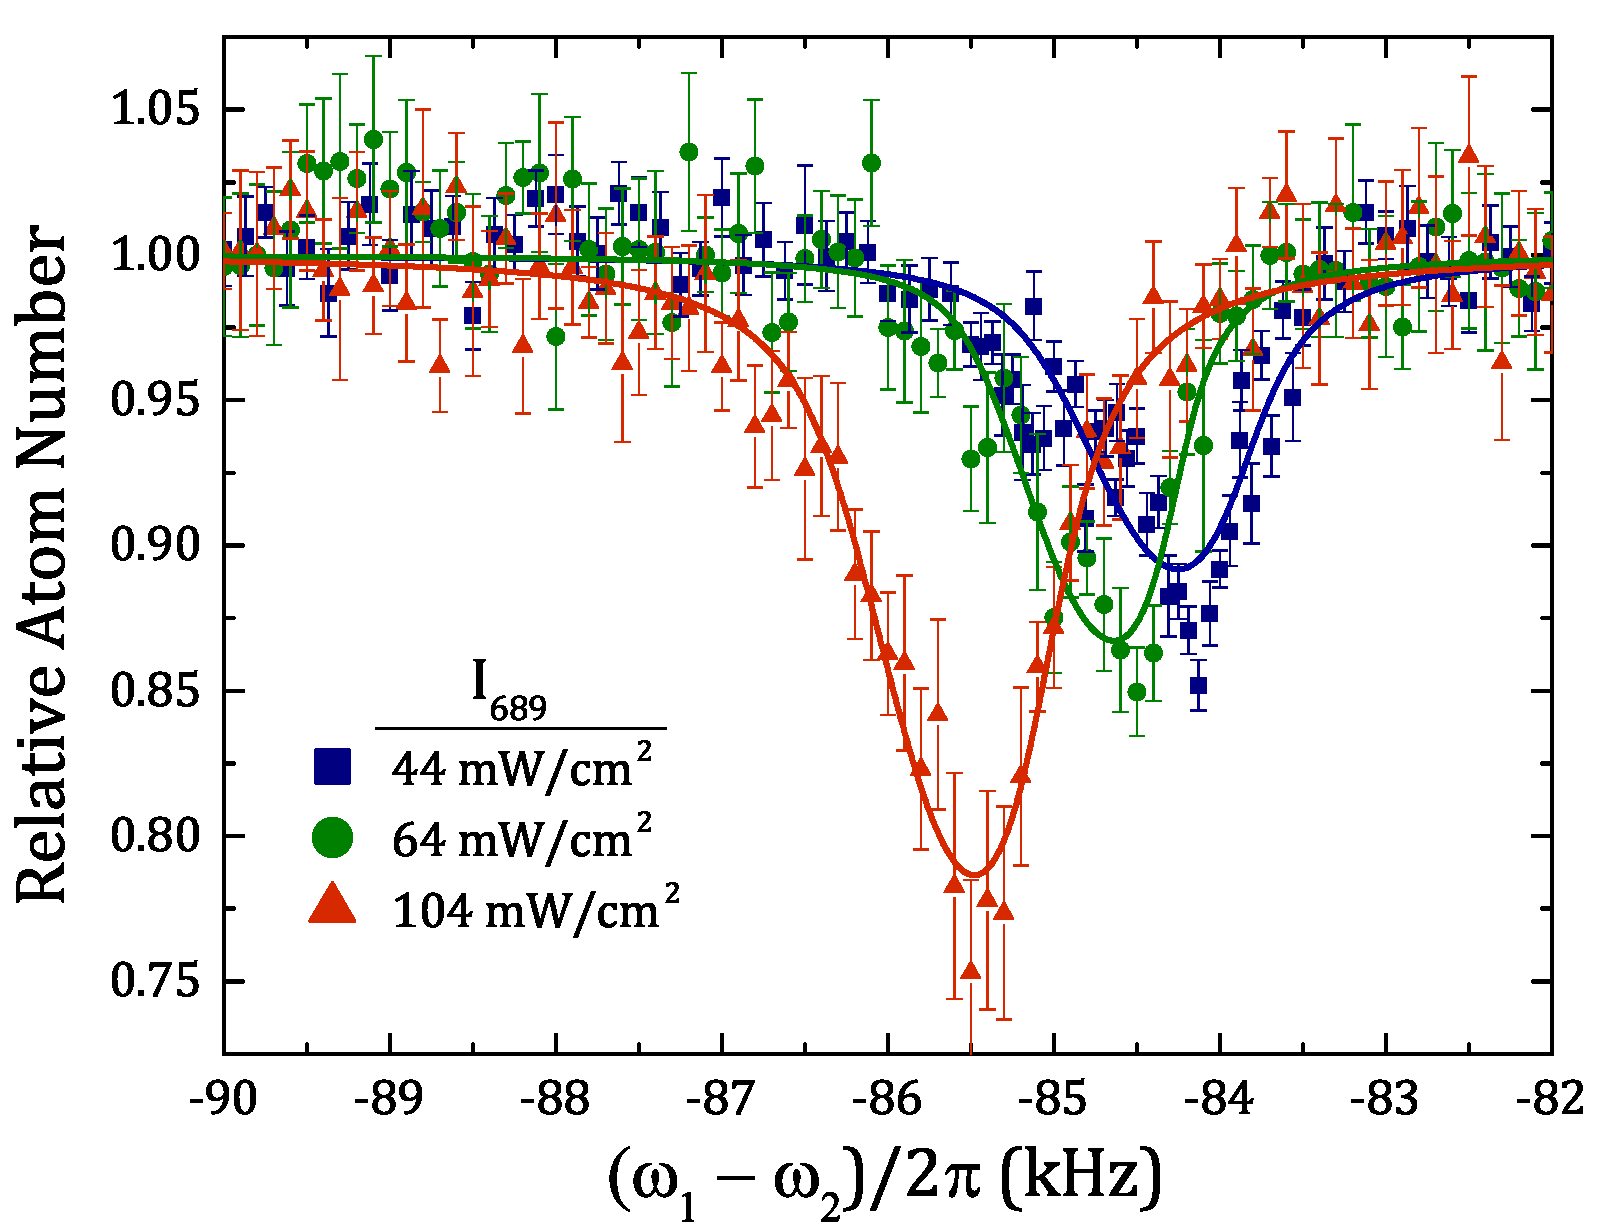
\includegraphics[width=\textwidth]{spectra_vary_689.pdf}}
	  \caption{Variation of 689 nm excitation}{Atom-loss spectra as a function of two-photon difference frequency $(\omega_1-\omega_2)/2\pi$ for intermediate detuning $\Delta_1/2\pi=-9$\,MHz and various 689-nm excitation laser intensities . Twice the single-beam intensity $I_{689}=2I$ is indicated in the legend.}
	 \label{Fig:SpectraVarying689Intensity}
	\end{figure}

	\begin{figure}
	\centerline{
	  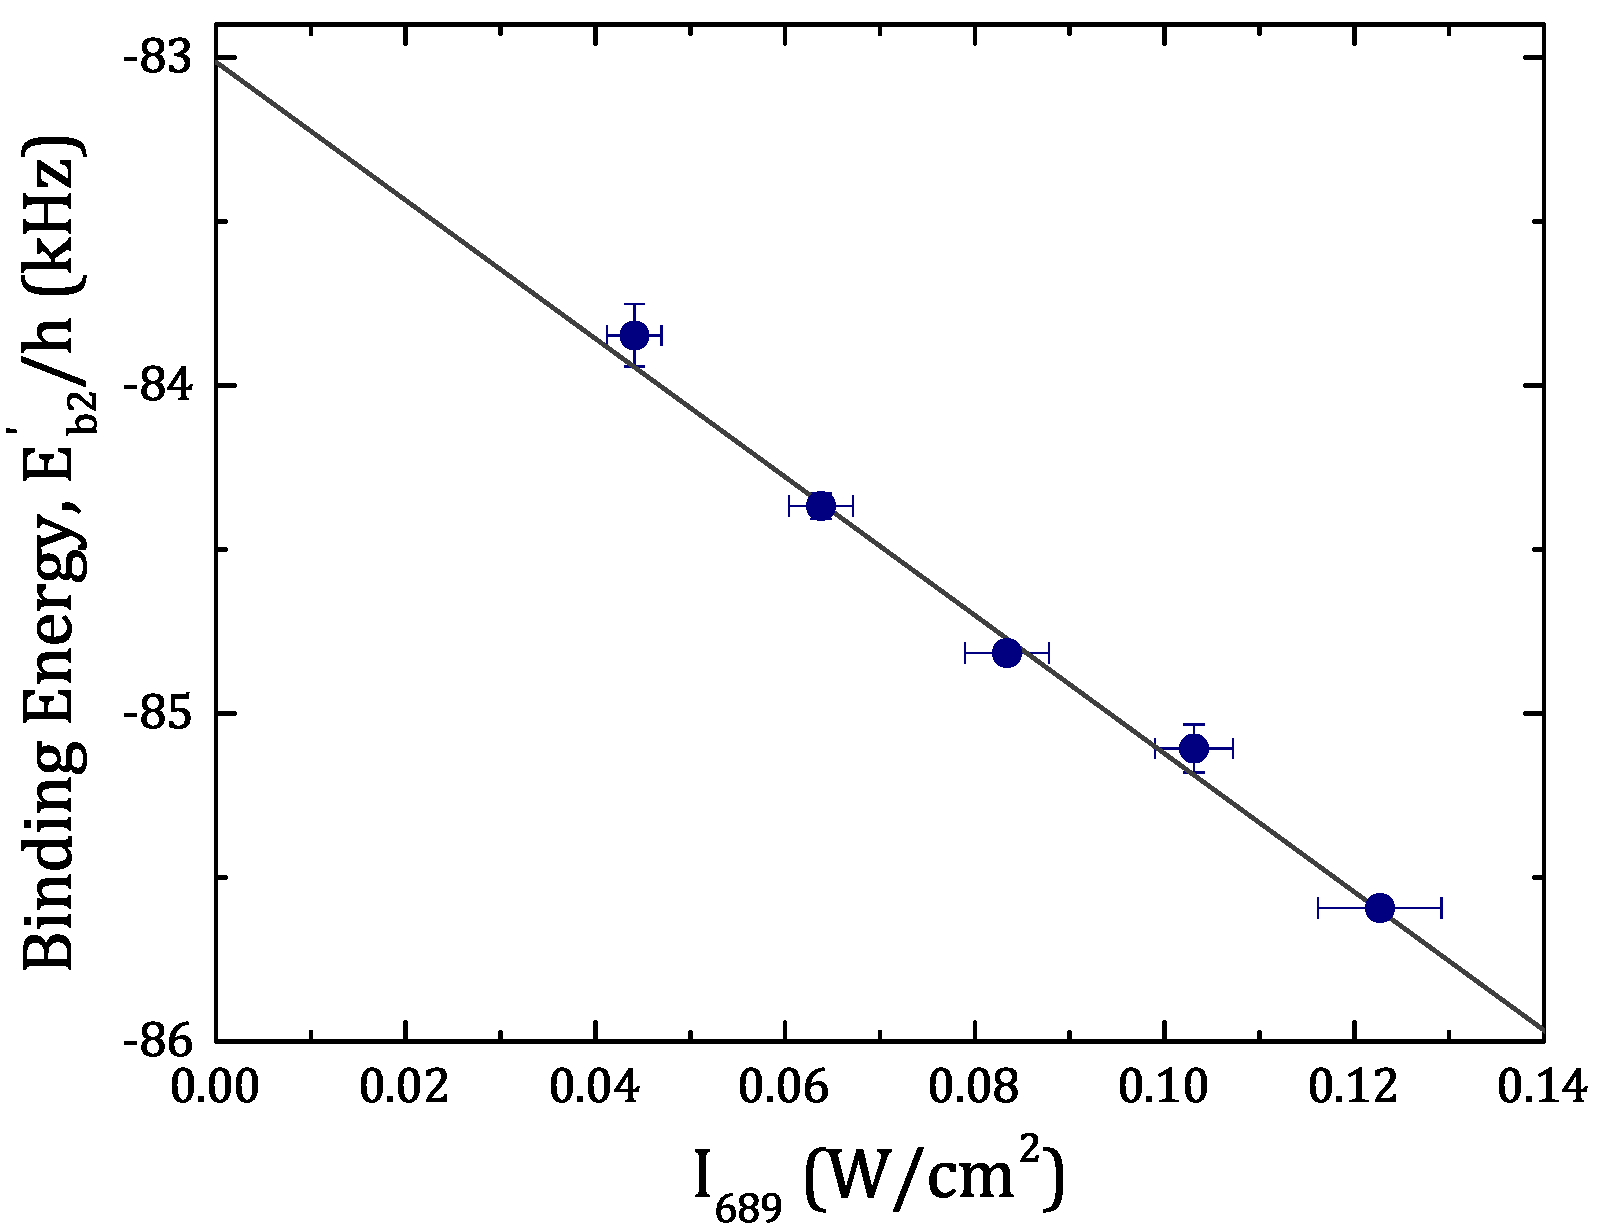
\includegraphics[width=\textwidth]{halo_susceptibility_689.pdf}}
	  \caption{Fit of 689 nm AC Stark shift}{Measured resonance position $E_{b2}'$ plotted versus twice the single-beam intensity $I_{689}=2I$ . The linear fit provides the AC Stark shift parameter $\chi_{689}$.}
	  \label{Fig:ShiftWith689Intensity}
	\end{figure}

The most significant perturbation to the resonance position is the AC Stark shift due to the excitation laser intensity, as shown in Fig.\ \ref{Fig:SpectraVarying689Intensity}.

For this data, the trap parameters, temperature ($T=30$\,nK), and initial peak sample density ($n_0=2\times 10^{12}$\,cm$^{-3}$) are held constant.

We vary the single-beam excitation intensity from $I=0.02-0.06$\,mW/cm$^{-2}$, and the excitation time is 50\,ms.

The observed shifts are comparable to the thermal width of the spectrum, allowing a precise determination of $\chi_{689}=-21(1)(2)$\,kHz/(W/cm$^{2})$ from a linear fit to the resonance positions, $E'_{b2}\propto h\chi_{689} I_{689}$ (Fig.\ \ref{Fig:ShiftWith689Intensity}).

The first quoted uncertainty is statistical and it arises from variations in parameters and fluctuations in the measured intensity during the scans.

The second value is systematic, reflecting uncertainty in laser-beam size and intensity profile at the atoms.

All parameters beside the 689-nm laser intensity are held fixed for this data set, and the AC Stark shift is not correlated with any other variable, such as density or trap intensity.

We thus obtain an accurate measure of $\chi_{689}$ without attempting to account for other systematic shifts of $E'_{b2}$ in this data.

A study of the dependence of $\chi_{689}$ on detuning from the excited molecular state will be discussed in Sec.\ \ref{sectionACStark}.

Broadening to the red of the spectrum reflects the distribution of atom-atom collision energies, while broadening to the blue is most sensitive to decay of the intermediate state ($\Gamma_L$) and the phenomenological broadening term $\gamma_{\text{eff}}$ [Eqs.\ (\ref{ApproxLorentzianQuantities-2Main}) and (\ref{equationApproxLorentzian})]. 

The long lifetime of the excited state and the significant detuning $\Delta_1$ result in a width $\Gamma_L(\epsilon)$ less than 5\,Hz for all conditions.

This is extremely small compared to observed width, which yields values of $\gamma_{\text{eff}}$ on the order of 300\,Hz.

We hypothesize that this width reflects decay of molecules in the electronic ground-state due to collisions with background atoms.







\subsection{Density-dependent frequency shift}
A shift of the two-photon resonance position is possible due to differing mean-field shifts of initial atomic and final molecular states arising from interaction with the background of ground-state atoms.

Such a shift would be proportional to the atom density and depend upon the $s$-wave scattering lengths for atom-atom and atom-dimer collisions, $a_{86}$ and $a_{\text{ad}}$ respectively.

This was observed in a Rb Bose-Einstein condensate (BEC) in \cite{wfh00}. For a non-degenerate gas, this effect yields $\chi_n=\hbar (\frac{a_{\text{ad}}}{\mu_{\text{ad}}}-4\frac{a_{86}}{\mu_{\text{aa}}})=\frac{\hbar}{m} (\frac{3 }{2}a_{\text{ad}}-8 a_{86})$, where $\mu_{\text{ad}}$ and $\mu_{\text{aa}}$ are the reduced masses for molecule-atom and atom-atom collisions respectively.

Note that the shift would vanish for $a_{\text{ad}}=(16/3) a_{86}$.

The largest density used in our experiment ($\sim 1\times 10^{12}\,\mathrm{cm}^{-3}$) is relatively low compared to typical BEC densities, and at this time we are unable to accurately measure a variation of resonance position with density.

However, the atom-atom scattering is close to resonance and thus Efimov physics can provide information on $a_{\text{ad}}$ \cite{bha07,nen17} and an estimate of the systematic error introduced by any residual density-dependent frequency shifts.

For a zero-range interaction, the atom-dimer scattering length is related to the atom-atom scattering length through the three-body Efimov parameter $\kappa_*$ according to \cite{bha07}
\begin{equation}\label{Eq:EfimovMoleculAtomScatteringLength}
  a_{\text{ad}}=a_{86}\left\{1.46 + 2.15 \mathrm{cot}[s_0 \mathrm{ln} (14.1\kappa_* a_{86}) ]\right\}
\end{equation}


where $s_0=1.006$ \footnote{The Efimov parameter is related to $E^0_{3b}$ through $\kappa_*=(m|E^0_{3b}|/\hbar^2)^{1/2}$, where $E^0_{3b}$ is the binding energy the lowest Efimov trimer would have in the case of resonant atom-atom interactions.}.

In principle, the atom-dimer scattering length can take any value.

However, for a deep atom-atom potential, such as for the ground-state strontium dimer \cite{skt10}, there is a universality of the three-body physics that sets $\kappa_*=0.226(2)/l_{\mathrm{vdW}}$ \cite{wie12}.

Here, $l_{\mathrm{vdW}}=\left({2\mu C_6}/{\hbar^2}\right)^{1/4}/2=74.6$\,$a_0$ is the van der Waals length associated with the $C_6$ coefficient of the long-range Sr$_2$ ground-state potential.

We use $C_6=3.03(1) \times 10^{-76}$\, J\,m$^6$ found from a fit of potential parameters to spectroscopic data \cite{skt10}, which is consistent with a recent \textit{ab initio} calculation \cite{zbb14}.

This yields $\kappa_*=5.72\times 10^7$\,m$^{-1}=(330\,a_0)^{-1}$. Equation (\ref{Eq:EfimovMoleculAtomScatteringLength}) then predicts $a_{\text{ad}}=6.4\, a_{86}$, which leads to a small density-dependent frequency shift parameter of $\chi_n=50\,\mathrm{Hz}/(10^{12}\,\mathrm{cm}^{-3})$.

A numerical calculation including a finite-range correction for the atom-atom interaction \cite{mwc17} results in $a_{\text{ad}}=3.5\, a_{86}$ and $\chi_n=-90\,\mathrm{Hz}/(10^{12}\,\mathrm{cm}^{-3})$.

Thus, a very small shift is expected for the densities used here.

We incorporate $\chi_n=0\pm 90 \,\mathrm{Hz}/(10^{12}\,\mathrm{cm}^{-3})$ as a set parameter in our model of the spectrum, where we set the systematic uncertainty to reflect the spread of theory predictions.

This uncertainty will be significant for our determination of the unperturbed halo binding energy.



%Figure \ref{Fig:SpectraDensityVariation} shows  spectra for different sample densities varying from $1-5\times 10^{12}$\,cm$^{-3}$, but the same trapping potential and excitation laser parameters. The samples are prepared by evaporating to a fixed trap depth and holding for 100-700\,ms to allow the atom number and peak density to decay due to three-body recombination, evaporation, and background-gas collisions.
%
%Figure \ref{Fig:ShiftWithDensity} shows the measured resonance frequencies as a function of the  peak density at the start of laser excitation. We observe a susceptibility $\chi_n=xx\pm yy$\,Hz/cm$^{-3}$, consistent with zero. The sample temperature also varies from $250-360$\,nK for this data, so there is some variation in the shift of the resonance from the trap-induced AC Stark shift, and we take that into account in our analysis and determination of the best value for $\chi_n$. (Can we state what that effect is?)
%The density in the experiments presented here is approximately 100 times less than in \cite{wfh00}, which precludes us from placing useful limits on $a_{ma}$ based on our measurements.








\subsection{AC Stark Shift due to Trapping Lasers}

There is an additional effect we considered which accounts for the spatial dependence of the AC Stark shift due to the variation in intensity of the 1064\,nm trapping laser.
We tested simulations accounting for this effect and found no noticeable deviations of the complete lineshape within our knowledge of the exact trapping potential.
Inclusion of this effect significantly increases the computation time of the lineshape so we approximated this effect by calculating a two-body weighted average intensity of the 1064\,nm laser to characterize the average shift experienced by the atoms due to the trapping potential.

	\begin{figure} 
	 \centerline{
	 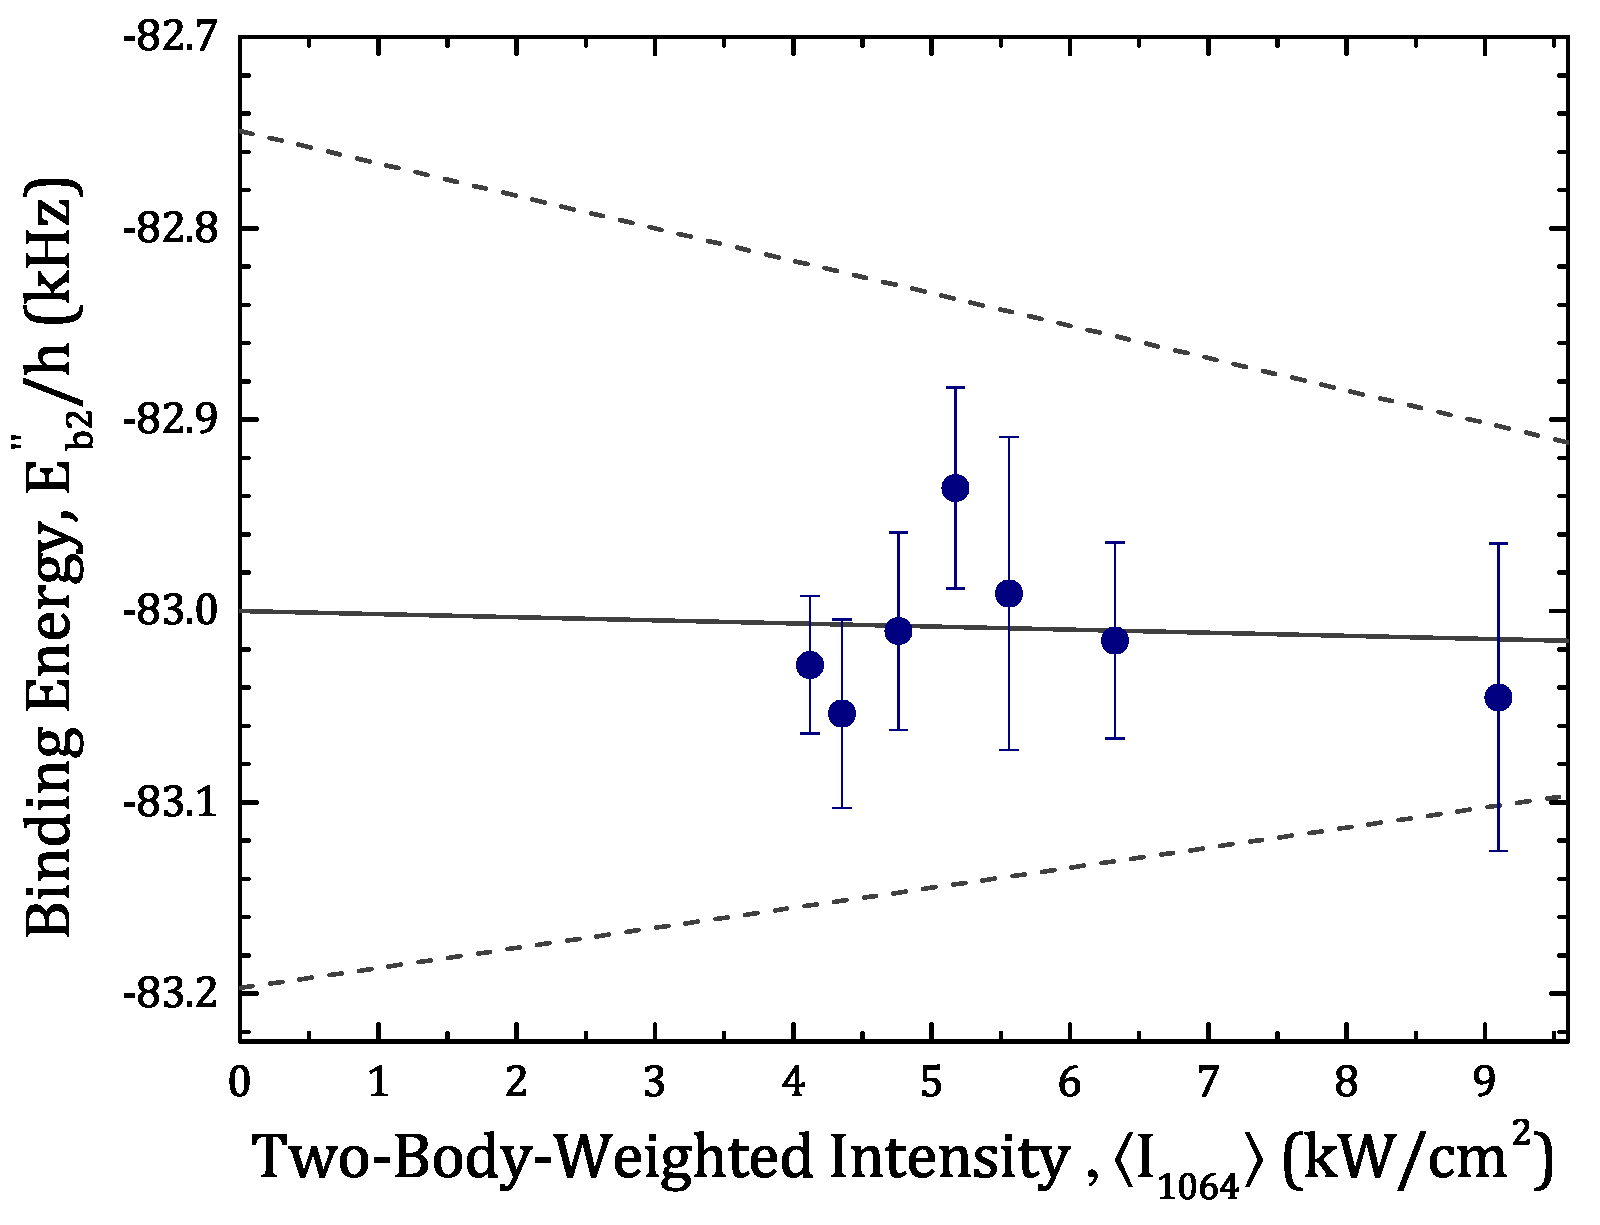
\includegraphics[width=\textwidth]{halo_susceptibility_1064.pdf}}
	  \caption{Measurement of halo state susceptibility, $\chi_{1064}$}{Measured resonance positions corrected for excitation-laser AC Stark shift and collisional frequency shift, $E_{b2}'-\chi_{689} I_{689} - \chi_{n}\langle n\rangle$, as a function of average trap laser intensity $\langle I_{1064} \rangle$ for the data such as in Fig. \ref{Fig:Spectraminus9MHzVaryTrapCold} . The trend line and confidence intervals are described in the text.}
	  \label{Fig:ShiftWithTrapIntensity}
	\end{figure}

With an accurate determination of $\chi_{689}$ and a value for $\chi_n$, we use the data shown in Fig. \ref{Fig:Spectraminus9MHzVaryTrapCold} to determine the susceptibility for the AC Stark shift from the trapping laser, $\chi_{1064}$, and the unperturbed halo binding energy $E_{b2}$.

Figure \ref{Fig:ShiftWithTrapIntensity} shows a plot of $E_{b2}'-\chi_{689}I_{689} - \chi_{\text{n}}\langle n\rangle$ versus $\langle I_{1064} \rangle $, where $E_{b2}'$ is the resonance position from each fit and $\langle ... \rangle $ indicates a weighted average of the quantity over the trapped sample, with a weighting given by the square of atom density.

This weighting reflects the contribution to photoassociative loss, a two-body process.

The plotted uncertainties in $E_{b2}'-\chi_{689}I_{689} - \chi_{\text{n}}\langle n\rangle$ are from statistical variation in the fit parameters.

The typical average density is $\langle n\rangle\approx 1\times 10^{12}$\,cm$^{-3}$. The linear fit function is to $E_{b2}+\chi_{1064}\langle I_{1064} \rangle $.

In addition to statistical uncertainty, we have systematic uncertainty from $\chi_{\text{n}}$ and treatment of the truncation of the collision-energy integral [Eq.\ (\ref{equationKeffective})].

The dashed lines shown in Fig. \ref{Fig:ShiftWithTrapIntensity} are resulting fits when the values of $E_{b2}'-\chi_{689}I_{689} - \chi_{\text{n}}\langle n\rangle$ are shifted by the sum of these systematic uncertainties.

The resulting value for the unperturbed binding energy is $E_{b2}/h=-83.00(7)(20)$\,kHz, where the first uncertainty is statistical, and the second is systematic.

We observe a susceptibility to $I_{1064}$ of $\chi_{1064}=0\pm 10$\,Hz/(kW/cm$^2$).


For two-photon spectroscopy to a weakly bound dimer, it is typical to neglect any potential AC Stark shift due to far-off-resonant trapping lasers because the atoms contribute to the overall polarizability approximately as free atoms.

But the high precision of our measurement allows us to detect a small shift.

This corresponds to a relative differential polarizability of ${\chi_{1064}}/{2\chi_{1064,\text{g}}g}={(\chi_{1064,b2}-2\chi_{1064,\text{g}}g}/{2\chi_{1064,\text{g}}g}\approx xx$.








\section{Discussion of the halo binding energy} \label{sec:lowE_alt}
%% paper

%The properties of halo molecules have been well studied \cite{kgj06}.
%One of the most interesting features is their universality, meaning that in the extreme, they can be characterized by a single parameter, the s-wave scattering length. For example,

In the limit of extremely small binding energy, and thus resonant atom-atom interactions, the binding energy of a halo molecule is approximately given by \cite{kgj06}
\begin{equation} \label{Eq:HaloEnergyNoCorrections}
	E_b=-\hbar^2/2\mu a^2.
\end{equation}


For interactions described at long-range by the van-der-Waals form, $V(r)=-C_6/r^6$, as with ultracold atoms, a convenient figure of merit for quantifying how accurate this simple expression should be is given by the ratio of the $s$-wave scattering length to the mean scattering length or interaction range, closely related to the van der Waals length through \cite{gfl93,cju05}
\begin{equation} \label{Eq:InteractionRangevdW}
  \bar{a}= l_{\mathrm{vdW}}\frac{\Gamma\left(\frac{3}{4}\right)}{\sqrt{2}\Gamma\left(\frac{5}{4}\right)}.
\end{equation}

%\begin{equation}\label{Eq:InteractionRangevdW}
%  \bar{a}=2^{-3/2}\frac{\Gamma\left(\frac{3}{4}\right)}{\Gamma\left(\frac{5}{4}\right)}\left(\frac{2\mu C_6}{\hbar^2}\right)^{1/4}.
%\end{equation}
%The universal relation $E_b=-\hbar^2/2\mu a^2$ is valid in general very close to a scattering resonance and over all values of scattering length for a zero-range delta-function pseudopotential \cite{hle57,cgj10}.

%\begin{equation}\label{Eq:HaloEnergyLeadingCorrection}
%-\hbar^2/2\mu(a-\bar{a})^2.
%\end{equation}
% This expression has been shown to be accurate for numerous magnetic Feshbach resonances \cite{cgj10,kgj06}, such as in $^{85}$Rb \cite{kgb03,ckt03}.
%Higher order corrections due to

Slightly away from resonance, corrections to the binding energy for the van der Waals potential were worked out in \cite{gao01,gao04}, yielding
\begin{equation} \label{Eq:BindingEnergyGao}
	E_{b2}=-\frac{\hbar^2}{2\mu(a-\bar{a})^2}\left[1+\frac{g_1\bar{a}}{a-\bar{a}}+\frac{g_2\bar{a}^2}{(a-\bar{a})^2} + ... \right],
\end{equation}


where $g_1=\Gamma(1/4)^4/6\pi^2-2=0.918...$ and $g_2=(5/4)g_1^2-2=-0.947...$. The range of validity of this expression is $a \gtrsim 2 \bar{a}$.

The accuracy of the first term in this expansion has been experimentally confirmed for various systems such as $^{85}$Rb \cite{ckt03,kgb03}, $^{40}$K \cite{rtb03,msg05} and $^{6}$Li \cite{bar05}.

This derivation of Eq.\ (\ref{Eq:BindingEnergyGao}) assumes that the influence of short-range physics, which can be expressed through a quantum defect, varies negligibly from threshold to the molecular binding energy.

We expect this to be an excellent approximation, since, as shown in Ref.~\cite{gao01} the corrections are typically less than about $1\%$ even for GHz binding energies.


%The long-range form of the interaction for s-wave collisions, which determines many aspects of atomic scattering at ultracold temperatures,  can be described with a van der Waals form, $V(r)=-C_6/r^6$. %where $C_6=3.03(1) \times 10^{-76} J m^6$  for Sr \cite{skt10}.
%Details of low energy scattering and near-threshold states for  a van der Waals potential have been well studied, and an important length scale was defined in \cite{gfl93} as the mean scattering length or interaction range \cite{cju05}
%\begin{equation}\label{Eq:InteractionRangevdW}
%  \bar{a}=2^{-3/2}\frac{\Gamma\left(\frac{3}{4}\right)}{\Gamma\left(\frac{5}{4}\right)}\left(\frac{2\mu C_6}{\hbar^2}\right)^{1/4},
%\end{equation}
%where $\mu$ is the reduced mass  and $\hbar$ is the reduced Planck's constant.

%$C_6=3.03(1) \times 10^{-76} J m^6$ \cite{skt10} and

%, where $a_0=5.29\times 10^{-11}$\,m is the Bohr radius.
%This value of $C_6$ is consistent with a recent \textit{ab initio} calculation \cite{zbb14}.

For ground-state $^{86}$Sr atoms, $\bar{a}=71.3$\,$a_0$.

The most accurate value available for the s-wave scattering length is $a=798 (12)$\,$a_0$ \cite{skt10}, satisfying the requirement of $a\gg \bar{a}$ for the least-bound state on the ground molecular potential to be a halo molecule.

Nonetheless, ${\bar{a}}/({a-\bar{a}})=.10$, and the corrections given by Eq.\ (\ref{Eq:BindingEnergyGao})are significant.

Figure \ref{Fig:HaloBindingEnergy} shows the importance of the correction terms.

	\begin{figure} 
	\centerline{
	  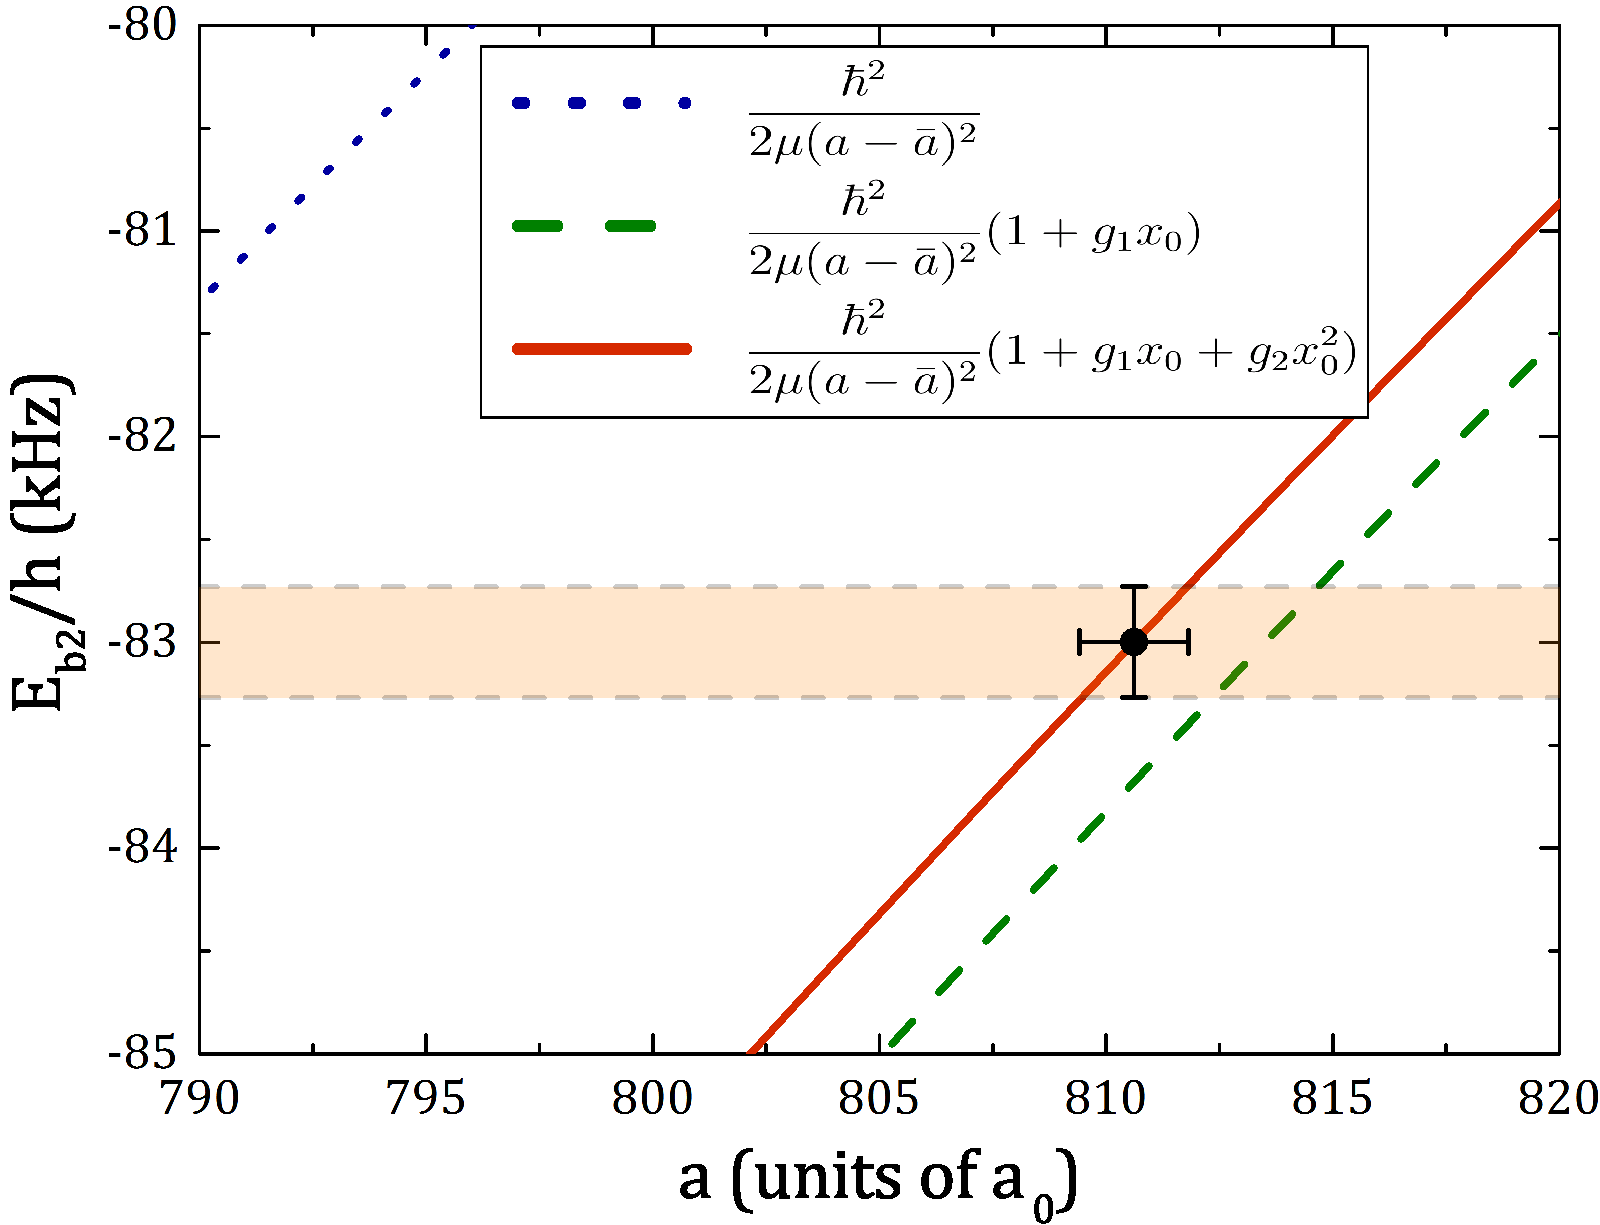
\includegraphics[width=\textwidth]{86_scattering_length.pdf}}
	  \caption{Determination of 86 scattering length}{Halo binding energy versus $s$-wave atom-atom scattering length for $^{86}$Sr . The shaded region indicates our experimental measurement. The lines are predictions of Eq.\ \ref{Eq:BindingEnergyGao} retaining up to the first, second, and third terms as indicated in the legend [$x_0={\bar{a}}/({a-\bar{a}})$]. The data point is the prediction of Eq.\ (\ref{Eq:BindingEnergyGao}) for the recommended value of the measured binding energy.}
	  \label{Fig:HaloBindingEnergy}
	\end{figure}

Equation (\ref{Eq:BindingEnergyGao}) and the previous best value of the scattering length \cite{skt10} predict a binding energy of $E_{b2}=-86(3)$\,kHz.

This agrees with our measurement, but by inverting Eq.\ (\ref{Eq:BindingEnergyGao}), we can use our increased accuracy in $E_{b2}$ to extract an improved value of the scattering length of $a=810.6(3)(9)$\,$a_0$, where uncertainties reflect statistical and systematic uncertainties in $E_{b2}$ respectively.

The next higher-order term in $x_0={\bar{a}}/({a-\bar{a}})$ is likely to introduce a correction on the order of $100$\,Hz in Eq.\ (\ref{Eq:BindingEnergyGao}), creating a systematic uncertainty in $a$ that is about one third of the uncertainty from our measurement.

%Uncertainty in $C_6$ corresponds to an uncertainty of $\sim 15$\,Hz in the binding energy, and is negligible.
	\begin{figure} 
	\centerline{
	  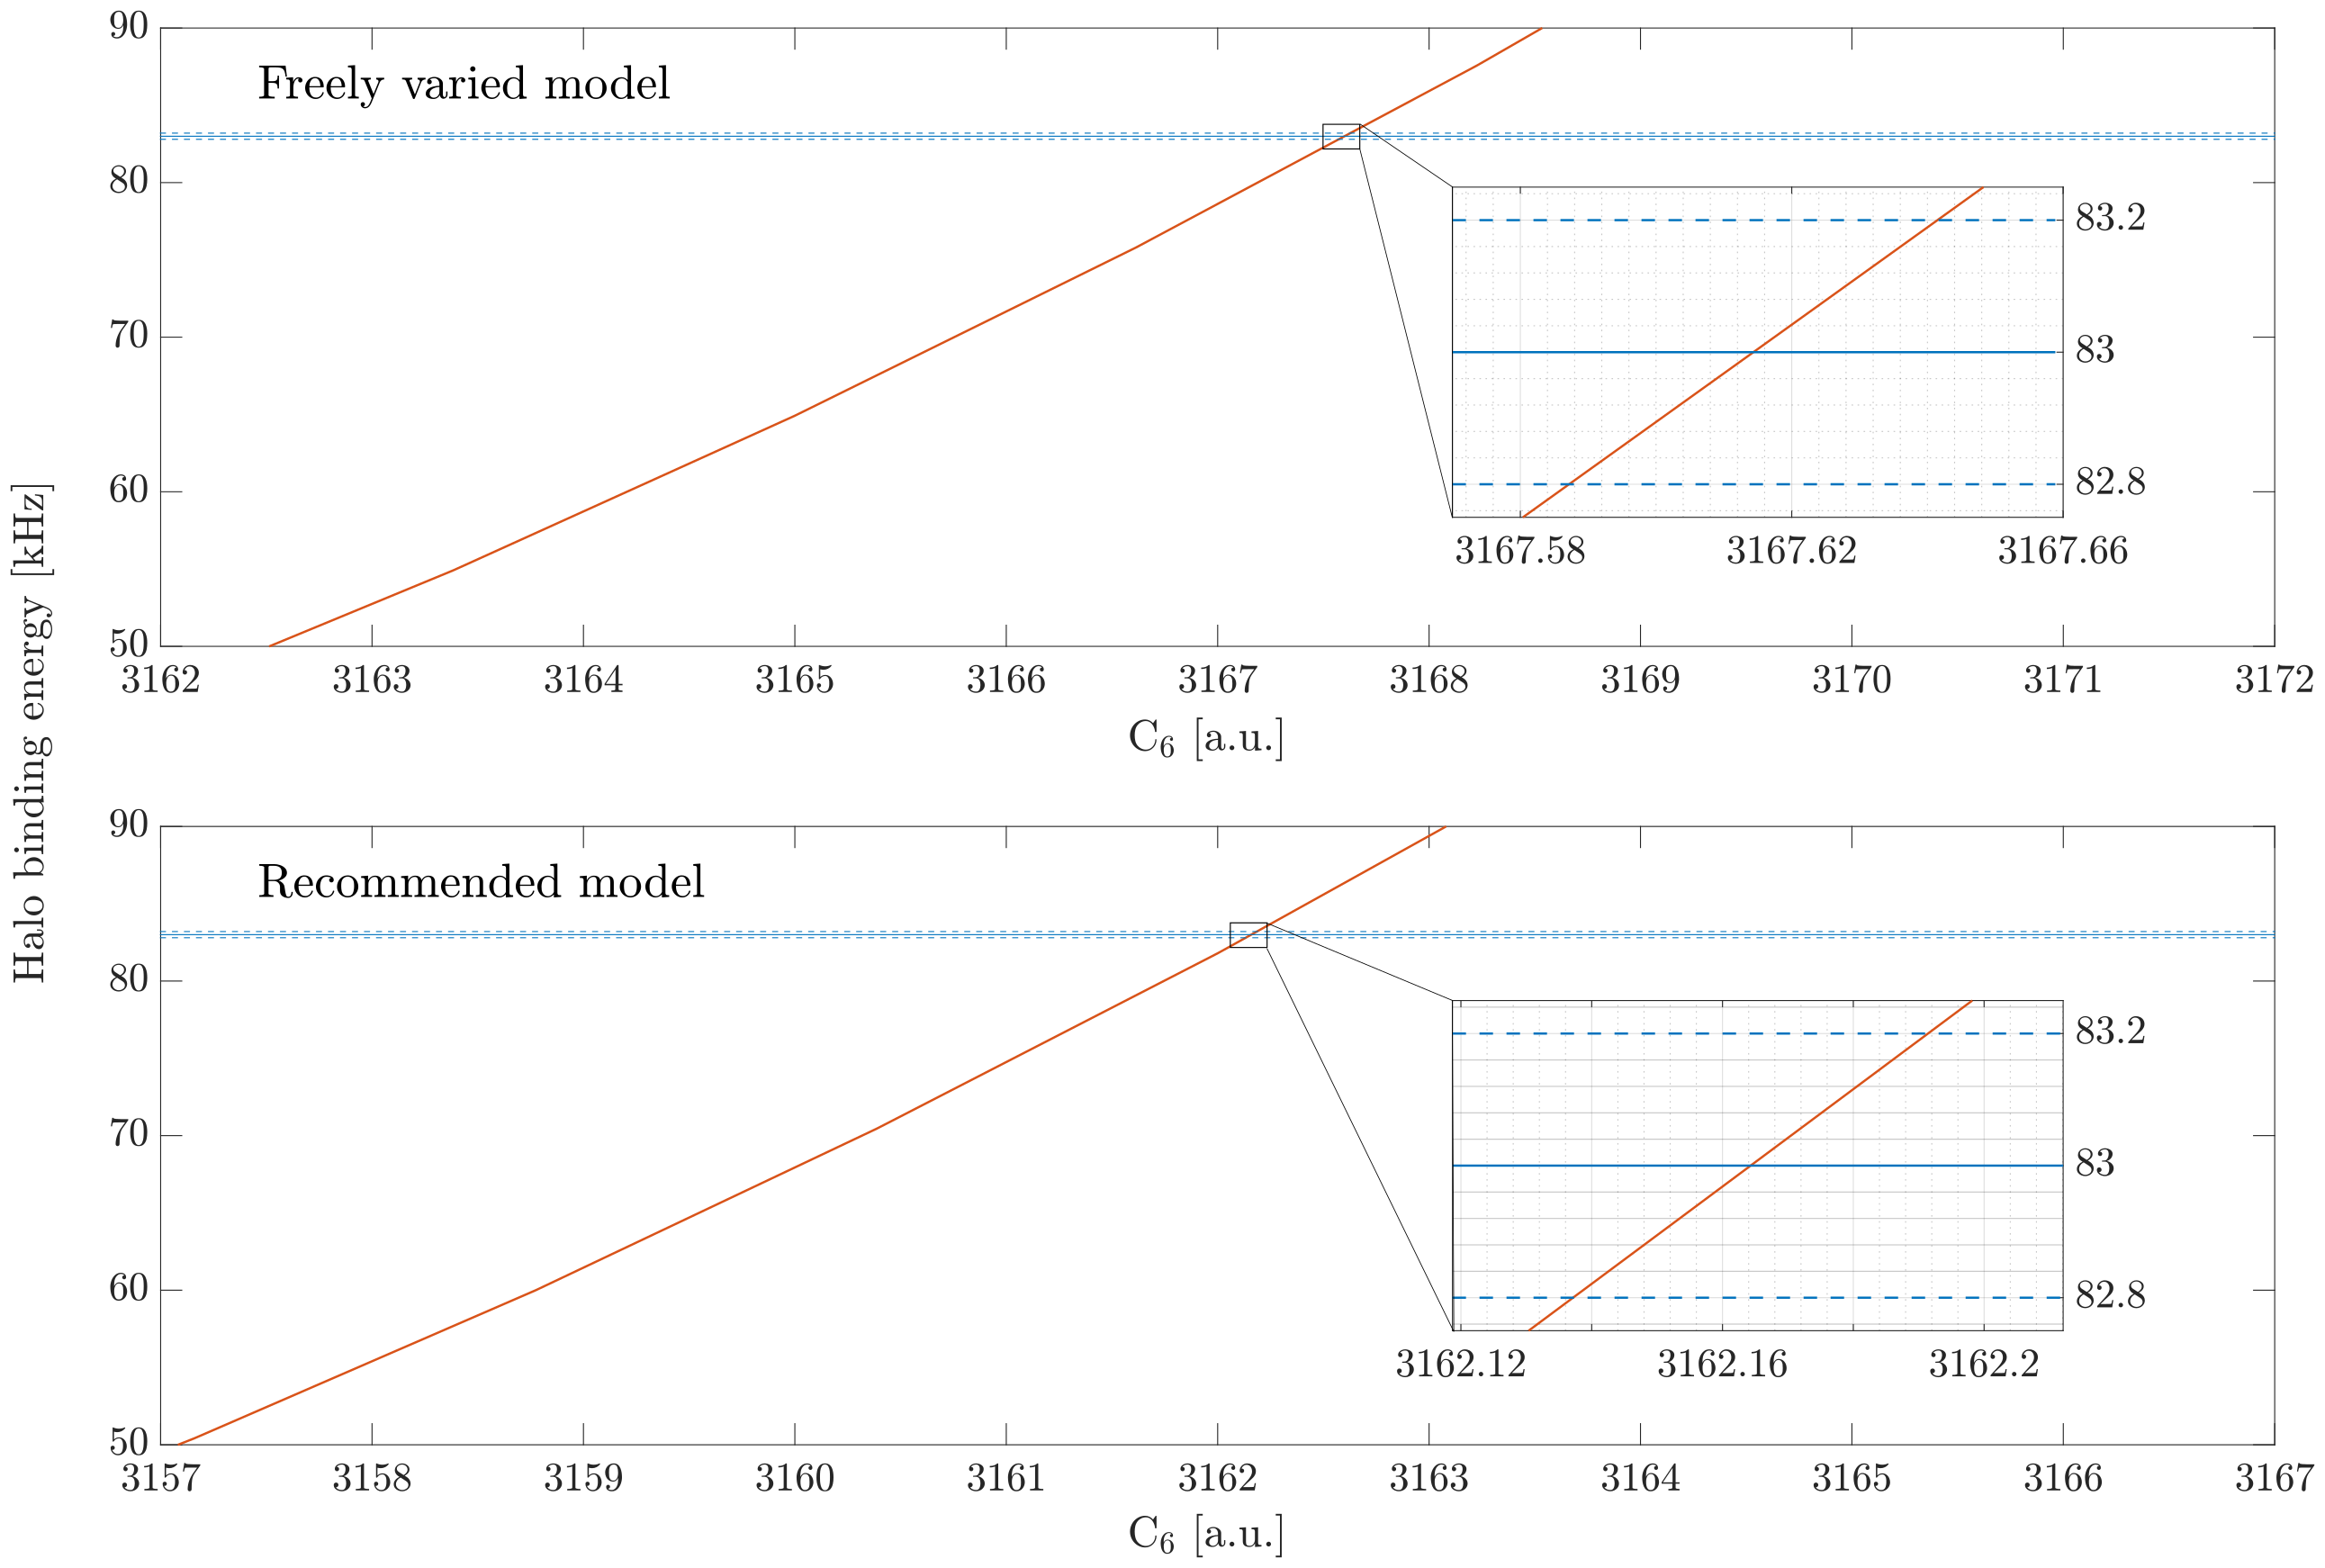
\includegraphics[width=\textwidth]{c6Comparison.png}}
	  \caption{Comparison of C$_6$ coefficient estimates}{Binding energy estimated from GF}
	  \label{fig:c6estimates}
	\end{figure}
	

We consider the collisional wavefunction and estimate the 86 scattering length via the position of the last node.
Using the two different values of C6 we calculate the wavefunction with a collision energy of 10nK to estimate the 
	\begin{figure} 
	\centerline{
	  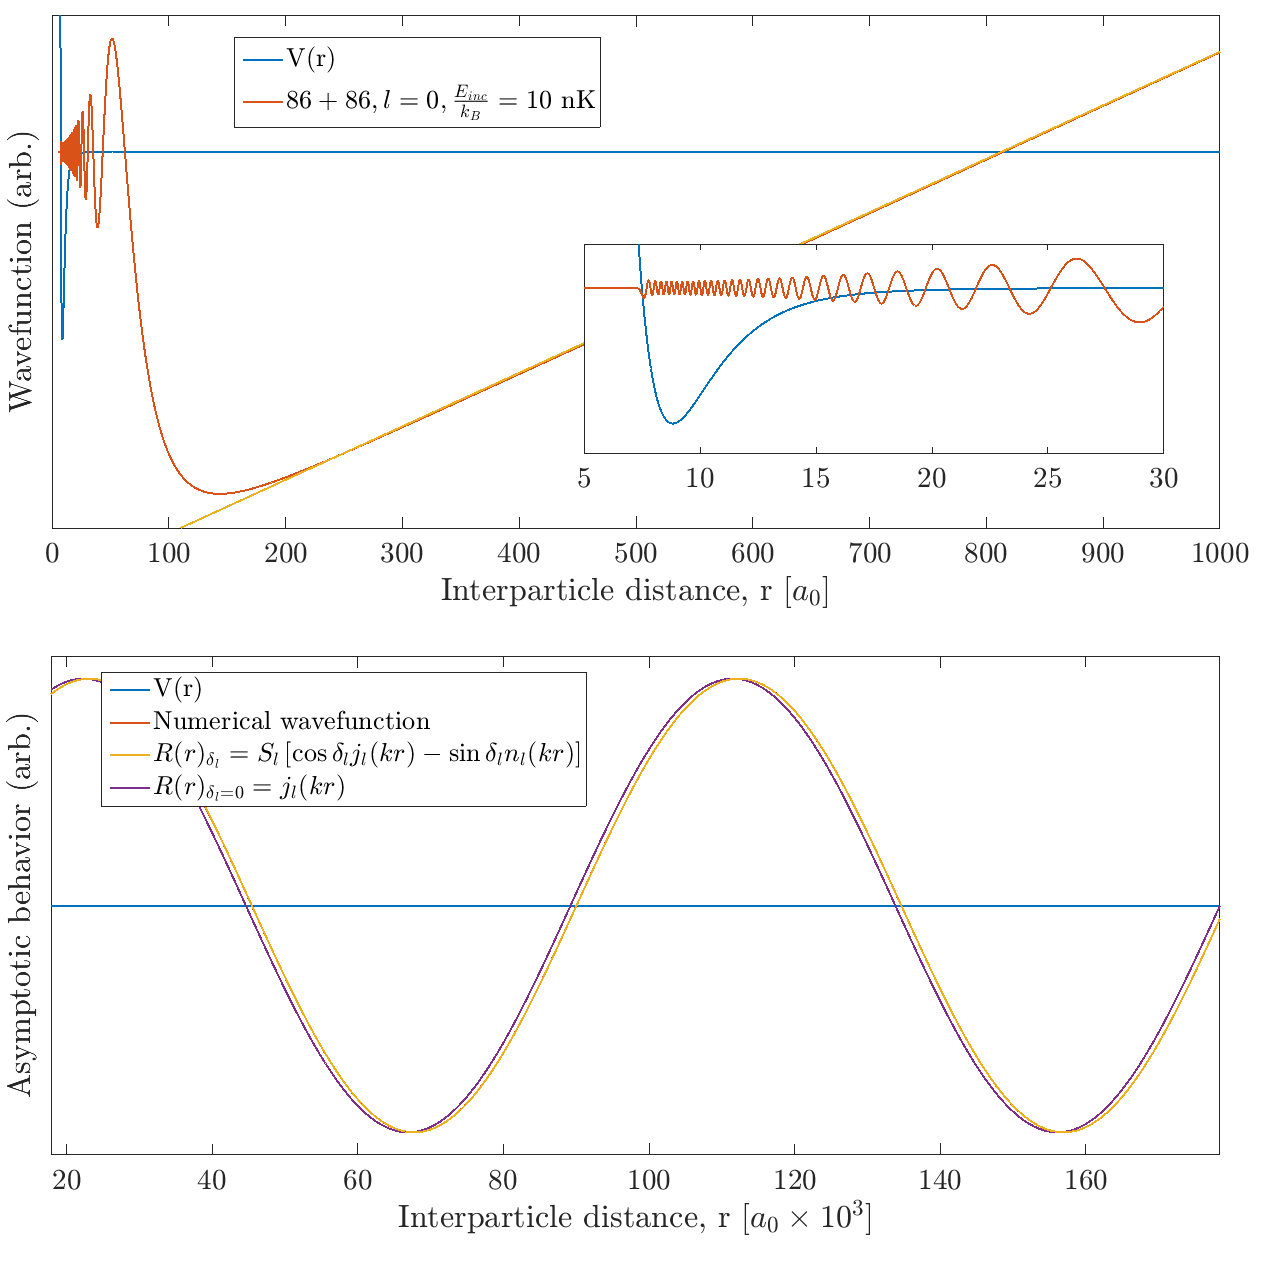
\includegraphics[width=\textwidth]{86collWF.png}}
	  \caption{$^{86}$Sr collision wavefunction}{Estimate scattering length via position of the last node.}
	  \label{fig:86CollWF}
	\end{figure}

Another way to estimate the scattering length is via a numerical integration of the ground state potential.

This method lets us quickly calculate the scattering length across a range of reduced masses in order to mass scale our model.

	\begin{figure} 
	\centerline{
	  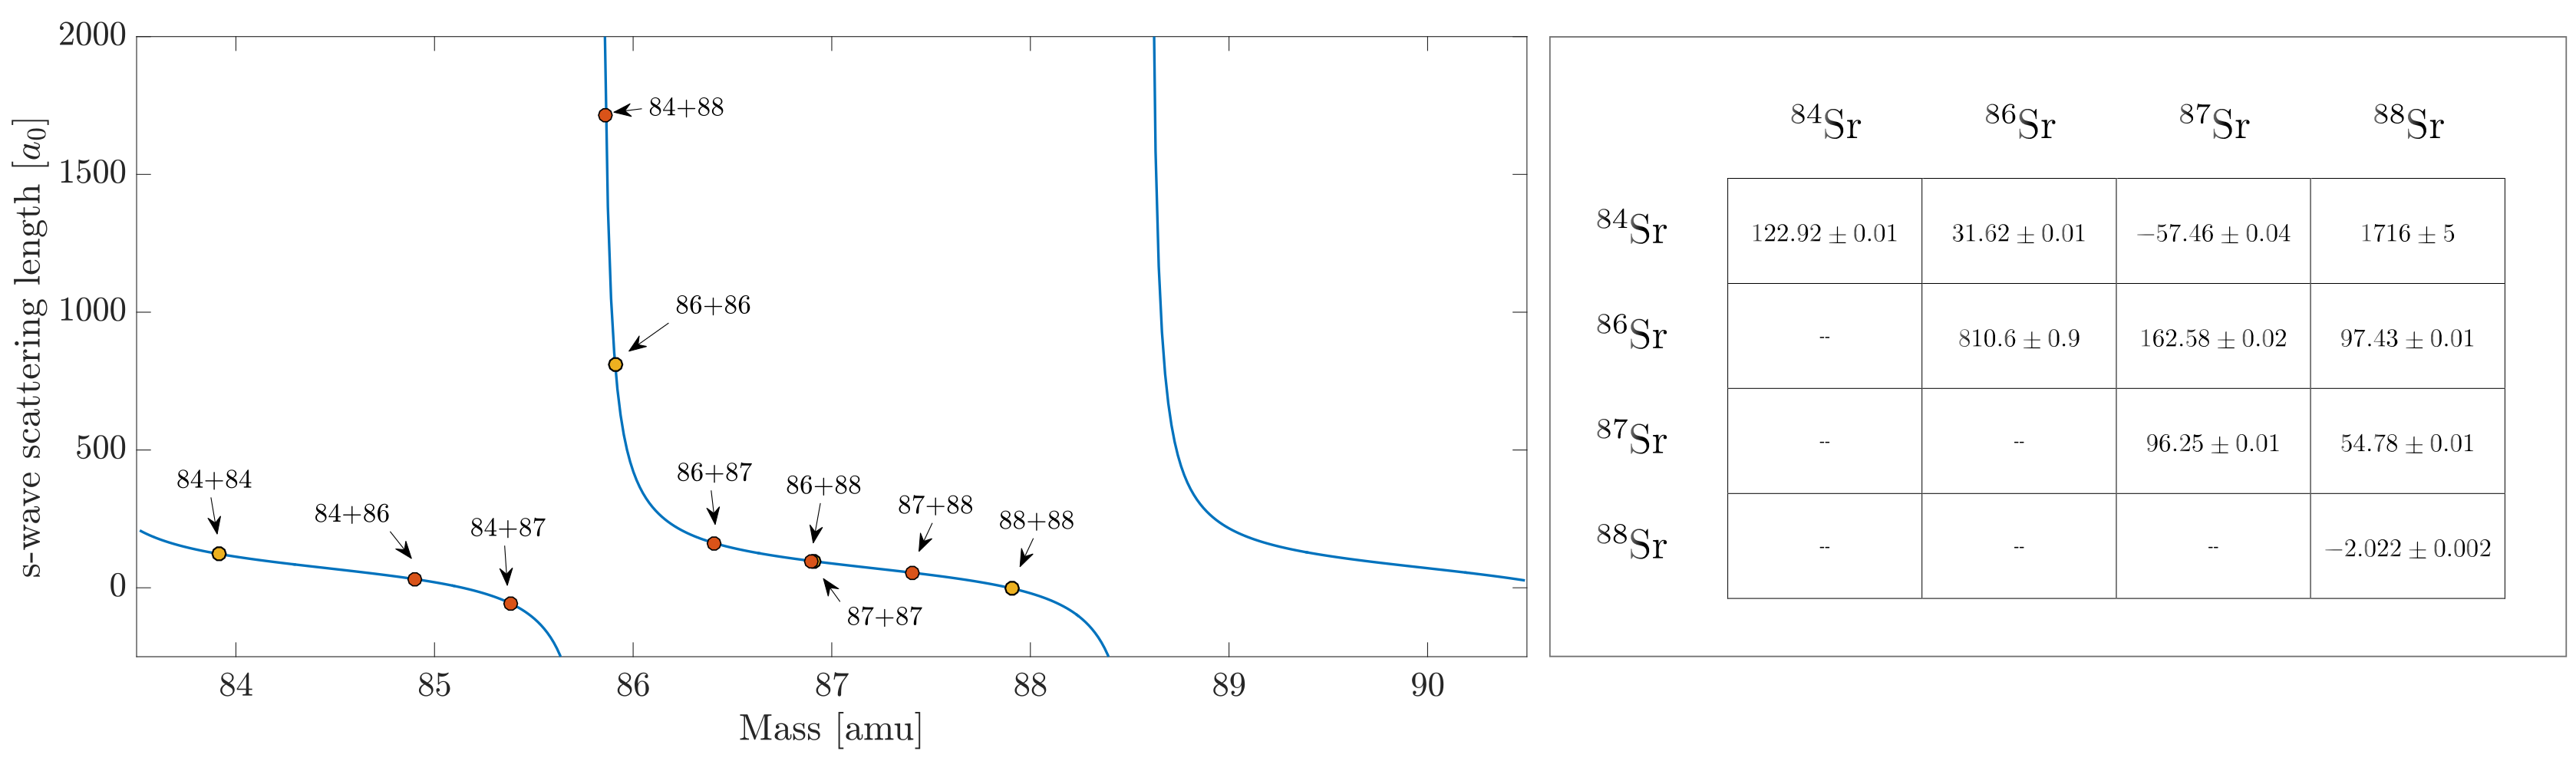
\includegraphics[width=\textwidth]{massScalingWithTable.png}}
	  \caption{Estimation of scattering lengths via mass scaling}{Using estimates of C$_6$ can mass scale }
	  \label{fig:massScaling}
	\end{figure}

%% %% %% %% %% %% %% %% %% %% %% %% %% %% %% %% %% %% %% %% %% %% %% %% %% %% %% %% %% %% %% %% %% %% %% %% %% %% %% %% %% %% %% %% %% %% %% %% 
%% other thoughts
From the formula for the line shape we can see that it depends on the spatial distribution of the atoms.

The standard approximation made when measuring these types of systems is to ensure loss does not cause heating of the atoms during photoassociation. 

Heating results in re-equilibration of the atomic density distribition, which in turn effects the rate of loss creation. 

Without independent controls to keep the system in thermal (and therefore spatial density) equlibrium.

What are the things the rate equation deals with?

We need the desnity distribution.

In a harmonic trap, there if a simp[le anayltic form to the density distribution of a thermal gas. 

From Mi's work (and others) we know that this is only an approximation that is valid when eta is approx greater than 4. 

When greater than 4 we can apply the high-eta approx and the trap frequencies along a particular direction reduce to <eq>.

However, the trap we did this experiment in were at eta's of 1 or less so we don't have an analytic solution to the spatial distribution.

Since this could be a problem we need to know what the trap looks like.

We measure trap oscillation freq. at several different powers and model the trap using the utility outlined somewhere else.

From the numeric model, we can define a spatially depedent eta which is determined by the local trap depth which is simply the difference between the local potential energy and the global depth.
This is illustrated in fig something.

The spatial information is not only important for the density determination, but also for the range of available thermal energies.

Consider two atoms near the local bottom of the trap. By definition, in equilibrium, a single atom may only have up to the trap depths worth of energy since any additional energy would result in its expulsion from the trap.

In this case, in a relative momentum frame, the allowed collision energies range from zero to two times the trap depth.

Similarly, as we move towards the edge of the trap the range of accessible collision energies shrinks.

This additional weighting factor may be viewed as having a local truncasted Boltzmann ditribution at every point in space. 

Normally the BZ dist goes to infinity but here we have a cutoff at 2 trap depeth.
The most naive approx would be to simply consider the BZ and harshly truncate at 2 trap depth. We tried this

We know this is unphysical since we should expect that the probability of observing a certain momenta at a certain point in space, should smoothly tend zero towards as we approach the edge of the trap.

To see what this looks like we (and determine how important the effect is) we rederive the relative momentum distribution.

<Some stuff about center of mass and relative>

What were all the cases and conclusions of having done this? Remember to consider what the different cases are.

If the total relative energy can be X then how does that get split up? Use the plots to show this limiting behavior.

Like if particle 1 has all the energy then there is only one possible value for particle 2 (and vice versa).

DERIVATION for truncated trap below

Need to lookup references for this molecular chaos assumption. What about egodicity? How to discuss that we may not be completely ergodic?

What does my potential look like? Can I make it a piecewise function? How should I introduce this part?

Where does the f equation come from? I believe this is just the normalized boltzmann factor for probability to occupy a particlar state.

\noindent
We can truncate this single particle distribution by 
\begin{equation}
\label{eq:trun_single_particle_prob}
		 f_{ \vec{r} }( \vec{p} ) = A \left(\frac{1}{2 \pi k_B T}\right)^{3/2} e^{\left(\frac{-p^2}{2 m k_B T}\right)} \Theta \left( \epsilon_{max} - U( \vec{r} ) - \frac{p^2}{2 m} \right)
\end{equation}

\noindent
where A is a normalization constant which ensures $\int_0^\infty f_{ \vec{r} }( \vec{p} )\,d \vec{p} = 1 $ and $\Theta(x)$ is the Heaviside function defined by

\begin{equation}
\label{eq:heaviside}
	\Theta(x)=
	\begin{cases}
		1 &\text{if } x \geq 0, \\
		0 &\text{if } x < 0
	\end{cases}
\end{equation}

We got a certain answer with the way shown in the paper.

We can also use a completely different method that ignores all the consdierations of the last few sections. As was done in the calcium paper, we could simply fit the blue edge of the feature using a model function which can capture the high level features of the lineshape. Get the same answer. SHOW PLOTS TO THIS AFFECT AND COMPARE

Maybe go a little into the isolated resonance model (or at least recall), then tie into how we can measure the susceptibility across several different detunings which can give us the coupling to intermediate level. The first order analysis of this data suggest a bound-bound rabi freuqnecy of \hl{BLAH}. 

Point out the curling up at the end and say how the simple isolated resonacne model cannot predict.

A full coupled channel calculation probably could but in the spirit of the Bohn and Julienne semi-classical approach, we set out to derive an approximate analytic expression to determine the binding energies.

THis is presented in the next chapter.

Lastly, we note that in the context of photoassociation, the center-of-mass component of Eq.\ref{eq:two_particle_prob_inf_atomFrame} is not typically considered as typical PAS experiments are performed utilizing broad dipole allowed transitions which have linewidhts much greater than the doppler width thus only the relative momentum between particles is important for determining the loss rate coefficient K discussed in \hl(somewhere). 

The case of PA using narrow intercombination line transitions found in alkaline-earth-metal atoms 

In general K is considered as a boltzmann average over a single loss rate constant
This can be seen in \cite{Ciuryo2004} Eq. 1 where the loss rate constant is given by

\begin{equation}
\begin{split}
\label{eq:ciuryo04_eq1}
		 K(\Delta,T) &= \left\langle\mathcal{K}(\Delta,\vec{P}_c,\vec{p}_r)\right\rangle \\
		 &= \int d^3\vec{P}_c \; f_M(\vec{P}_c) \int d^3\vec{p}_r \; f_{\mu}(\vec{p}_r) \; \mathcal{K}(\Delta,\vec{P}_c,\vec{p}_r)
\end{split}
\end{equation}


To this end we can integrate out the center of mass component to obtain the distribution most typically relevant to photoassociation.

By the time I've gotten to this I have already introduced K and that is not what I wanted to do. 

conclusion
here is the modified version of K we need for a trap that has a truncated energy disttribution

to get there
normal version of K is \hl{given in ch3}
this K can be given in terms of f? 
this version of f is given in the appendix
	why do I integrate out the com component?

typical PAS experiments utilize dipole allowed transitions which have linewidths many times larger than the 

We now perform a change of variables using Eq. and Eq.\ref{eq:two_particle_prob} can be rewritten as 

In the s-wave limit I need to write K as a function of f(p) (should do this in the appendix proof and reference in body). Given the form of the loss rate constant K, our problem reduces to determining the form of f(p) when eta is finite.

Ok, so need to reference \cite{Ciuryo2004} to motivate usage of center of mass.
Then use \cite{Nicholson2015a} Eq. 43 to reference the particular form 


what is the throughline I want to make? Develop K$_{in}$ $\rightarrow$ recast in terms of P distribution $\rightarrow$ show how we can replace the normal dist with a truncated dist $\rightarrow$ explore the effects of that truncation 


%To prove this assumption I want to show that using the square step I can get the same equations like in Eq. 1 of the 99 paper. Then once we know the infinite energy behavior (valid for only a particular portion of energy due to s-wave constraint) then we can ask what happens if f(p) is truncated. 
